%% Beginning of file 'SN\,2020jgb.tex'
%% using aastex version 6.3
\documentclass[twocolumn]{aastex631}

\newcommand{\sn}{SN\,2020jgb}
\newcommand{\trmax}{$t_{r_\mathrm{ZTF},\mathrm{max}}$}
\newcommand{\tfl}{$t_\mathrm{fl}$}
\newcommand{\Mch}{$M_\mathrm{Ch}$}
\newcommand{\kms}{$\mathrm{km}\,\mathrm{s}^{-1}$}
\newcommand{\adam}[1]{\textcolor{red}{[AAM: #1]}}
\newcommand{\chang}[1]{\textcolor{blue}{[Chang: #1]}}

\shorttitle{\sn}
\shortauthors{Authors et al.}
\graphicspath{{./}{figures/}}

\begin{document}

\title{\sn}

\author{Authors}
\affiliation{Center for Interdisciplinary Exploration and Research in Astrophysics (CIERA), Department of Physics and Astronomy, Northwestern University, 1800 Sherman Road, Evanston, IL 60201, USA}

\begin{abstract}
I am an abstract.
\end{abstract}

\keywords{We are the keywords}

\section{Introduction} \label{sec:intro}
It has been clear for decades that Type Ia Supernovae (SNe Ia) are caused by the thermonuclear explosions in carbon-oxygen (C/O) white dwarfs (WDs) in binary systems \citep[see][for a review]{Maoz_2014}. Nevertheless, the nature of the binary companion, as well as how it ignites the WD, remains highly uncertain. 

The helium-shell (He-shell) double detonation (DDet) scenario is one of the most promising channels to produce SNe Ia. In this scenario, the WD accretes from a companion to develop a helium-rich shell, which, once becomes massive enough, could detonate. Such a detonation sends a shock wave into the C/O core to trigger a runaway thermonuclear explosion and inevitably destroy the whole WD \citep{Nomoto_1982a, Nomoto_1982b, Woosley_1986, Livne_1990, Woosley_1994, Livne_1995}, even when the WD is below the Chandrasekhar mass (\Mch).

There are several observational benchmarks for He-shell DDet triggered SNe. Shortly after the ignition of the shell, the decay of radioactive material in the helium ashes may power a detectable flash \citep{Woosley_1994,Fink_DD_2010,Kromer_DD_2010}. The Fe-group elements in the ashes will blanket blue photons with wavelengths $\lesssim$5000\,\AA\ \citep{Kromer_DD_2010}, the duration of which depends on the mass of the He-shell. For thick enough shells, \citet{Boyle2017_Helium} suggest that the unburnt helium could provide observational signal in near infrared (NIR) spectra, and \citet{polin_nebular_2021} predict significant [\ion{Ca}{2}] emission in the nebular phase of the SNe.

Using different combos of He-shell mass and C/O core mass, one can reproduce a variety of observables in `normal' SNe Ia with typical luminosities and spectral features near peak light, or peculiar sub-luminous ones \citep{polin_observational_2019}. 

For the DDet SNe that show `normal' characteristics near their peaks, the mass of the He-shell is expected to be low \citep[$\lesssim$0.03\,$\mathrm{M_\odot}$;][]{Kromer_DD_2010,Sim_2010,Shen_DD_2018,polin_observational_2019}. The first DDet candidate with a thin He-shell is SN\,2016jhr \citep{jiang_16jhr_2017}, which exhibits an early red flash and keeps a red $g-r$ color throughout its evolution, though it show a typical absolute magnitude at peak ($M_g\approx-19$) for normal SNe Ia. The multi-band light curves involving the early flash and the major peak, as well as the optical spectrum close to the peak light, could be simultaneously fit by a near-\Mch\ DDet model (a 1.38\,$\mathrm{M_\odot}$ C/O core and a 0.03\,$\mathrm{M_\odot}$ He-shell). Recently, a thinner He-shell is discovered in SN\,2018aoz \citep{Ni_2022}, a SN Ia showing a rapid redward color evolution within $\approx$12\,hr after the first light, which could be explained by a sub-\Mch\ DDet model (a 1.05\,$\mathrm{M_\odot}$ C/O core and a 0.03\,$\mathrm{M_\odot}$ He-shell). After this red excess the photometry evolution is consistent with normal SNe Ia, when the ashes of the thin He-shell becomes optically thin. To date, only a small fraction of SNe Ia have been discovered early enough for possible detection of early flashes \citep[e.g.,][]{Deckers_2022}. While there could be a large underlying population of normal SNe Ia triggered by He-shell DDet, it is hard to prove so.

In contrast, if the He-shell mass is much greater than 0.03\,$\,\mathrm{M_\odot}$, the ashes of the He-shell detonation could remain optically thick in a much more extended phase, resulting in the red color and low luminosity near peak light. SN\,2018byg \citep{de_18byg_2019} is a prototype of thick He-shell DDet SNe. During the late stages of preparing for this paper, \citet{Dong_16dsg_2022} presented another thick shell He-shell DDet candidates, SN\,2016dsg, accompanied with an archival transient OGLE-2013-SN-079 \citep{Inserra_OGLE13_079_2015}. All three candidates are faint, red, and show strong line-blanketing near peak lights. \citet{Dong_16dsg_2022} also report tentative detection of unburnt helium in SN\,2016dsg. The small sample size to date suggests thick shell events might be intrinsically rare.

It has been suggested that some, if not all, of the calcium-rich (Ca-rich) gap transients, a population of faint SNe with conspicuous [\ion{Ca}{2}] emission in the nebular phase, also arise from He DDet \citep{Dessart_2015,de_Ca_rich_2020,polin_nebular_2021}. A subclass of Ca-rich transients resemble SNe Ia near peak lights (termed Ca-Ia objects), marked by the strong \ion{Si}{2} absorption and the absence of optical \ion{He}{1} lines. There are only two Ca-Ia objects \citep[SN\,2016hnk and SN\,2019ofm;][]{de_Ca_rich_2020}, both showing significant line-blanketing in spectra, and hence could be He-shell DDet objects. Nonetheless, they also exhibit properties of other types of sub-luminous SNe Ia, such as the strong \ion{O}{1} absorption widely seen in 91bg-like objects \citep{Filippenko_91bg_1992} but not in other He-shell DDet candidates. \citet{galbany_16hnk_2019} argue that SN\,2016hnk is also consistent with a 91bg-like object arising from the deflagration of a near-\Mch\ WD. In a word, the nature of Ca-Ia objects remain ambiguous. \textbf{Mention red Ca-Ib/c?}

%SN\,2016hnk as a sub-\Mch\ He-shell DDet \citep{jacobson-galan_16hnk_2020} (0.85\,$\mathrm{M_\odot}$+0.02\,$\mathrm{M_\odot}$) or a near-\Mch, 91bg-like object 

In this paper, we present the observations of another promising candidate of a thick He-shell DDet SN, \sn. This peculiar SN Ia highly resembles SN\,2018byg in photometric and spectroscopic properties, and exhibits a remarkable feature in the NIR spectrum that could be attributed to the unburnt helium. In Section~\ref{sec:obs} we report the observations of \sn, which are analyzed in Section~\ref{sec:analysis}, where we show its similarities with other He-shell DDet SNe and discuss the tentative \ion{He}{1} absorption features. We use a grid of DDet models to fit the data of \sn, and present the results in Section~\ref{sec:model}. In Section~\ref{sec:host} we discuss the diversity in the host environments of DDet events. We draw our conclusions in Section~\ref{sec:discussion}.

\section{Observations} \label{sec:obs}
\subsection{Discovery}

%\chang{I do not have access to your .bib file, so my addition of references will be a little mixed and matched.}

\sn\ was first discovered by the Zwicky Transient Facility \citep[ZTF;][]{ZTF2019a,ZTF2019b} on 2020 May 03.463 UT (MJD 58972.463) with the 48-inch Samuel Oschin Telescope (P48) at Palomar Observatory. The automated ZTF discovery pipeline \citep{Masci_2019} detected \sn\ using the image-differencing technique of \citet{Zackay_imagesub_2016}. The candidate passed internal thresholds \citep[e.g.,][]{Mahabal_ZTFML_2019, Duev_ZTFML_2019}, leading to the production and dissemination of a real-time alert \citep{Patterson_ZTFalert_2019} and the internal designation ZTF20aayhacx. It was detected with $g_\mathrm{ZTF} = 19.86 \pm 0.15\,$mag at $\alpha_\mathrm{J2000}=17^\mathrm{h}53^\mathrm{m}12^\mathrm{s}.651$, $\delta_\mathrm{J2000}=-00^\circ51'21''.81$ and announced to the public in \citet{Fremling_report_2020}. The host galaxy, PSO J175312.663+005122.078, is a dwarf galaxy, to which \sn\ has a projected offset of only $0.3''$. The last non-detection limits the brightness to $r_\mathrm{ZTF} > 20.7$\,mag on 2020 April 27.477 (MJD 58966.477; 5.99\,days before the first detection). This transient was classified as a SN\,Ia in \citet{TNS_2020}.% \chang{These details are not given in that report, I would simply say - classified as a SN\,Ia in ...}

\subsection{Host Galaxy Observations}
We obtained a DEIMOS spectrum of the host galaxy, PSO J175312.663+005122.078, on 2022 March 31. The host exhibits strong, narrow emission lines including H$\alpha$, H$\beta$, [\ion{N}{2}] $\lambda$6583, [\ion{O}{3}] $\lambda$5007, and [\ion{S}{2}] $\lambda$6716 \& $\lambda$6731. By fitting all these emission features with Gaussian profiles we obtain an average redshift of $z=0.0309\pm0.0003$. With the diagnostic emission line equivalent width ratios ($\log$~[\ion{N}{2}]/H$\alpha=-1.19\pm0.07$ and $\log$~[\ion{O}{3}]/H$\beta=0.53\pm0.06$), the host is consistent with star-forming galaxies in the BPT diagram \citep{BPT_1981, Veilleux_1987}. 

To get the distance modulus to \sn, we use the 2M++ model \citep{Carrick2015_2M++} to obtain a peculiar velocity towards its host galaxy, PSO\,J175312.663+005122.078, to be 179\,\kms. This, combined with the recession velocity in the frame of the cosmic microwave background\footnote{See \url{https://ned.ipac.caltech.edu/velocity_calculator}.} (CMB) $v_\mathrm{CMB}=9136$\,\kms, yields a net Hubble recession velocity of $9307$\,\kms, with a systematic uncertainty of 250\,\kms \adam{Dominated by the 2M++ cosmic flow?}. Adopting $H_0=70$\,\kms\,Mpc$^{-1}$, $\Omega_M=0.3$, and $\Omega_\Lambda=0.7$, we estimate the luminosity distance to \sn\ to be 136.1\,Mpc, which yields a distance modulus of $\mu=35.66\pm0.06$.

\subsection{Optical Photometry}
\sn\ was monitored in the $g_\mathrm{ZTF}$ and $r_\mathrm{ZTF}$-bands by ZTF as part of its ongoing Northern Sky Survey \citep{ZTF2019a}. %\chang{The g and r bands used by ZTF are non-standard (relative to SDSS). To make this very clear to the reader, I often write $g_\mathrm{ZTF}$ to be explicitly clear, though that is not necessary.} 
We adopt a Galactic extinction of $E(B-V)=0.404\,$mag \citep{Schlafly2011}, and correct all photometry using the \citet{Fitzpatrick1999} extinction model. We assume there is no additional extinction in the host galaxy. This assumption is supported by the lack of \ion{Na}{1} D absorption at the redshift of the host galaxy, though see \citet{Poznanski_2011} for caveats on the use of \ion{Na}{1} D absorption as a proxy for extinction. 

The forced photometry light curves\footnote{\url{https://web.ipac.caltech.edu/staff/fmasci/ztf/forcedphot.pdf}} in absolute magnitudes in $g_\mathrm{ZTF}$- and $r_\mathrm{ZTF}$-bands are shown in Figure~\ref{fig:photometry}, in which we show all the measurements with $\mathrm{SNR}>2$. The light curves are reduced using the pipeline from Miller et al. (2022, in preparation). %\chang{Should point to ZTF forced light curve service as a reference here - probably also make sense to cite Miller et al. in prep since I made the light curve}

\begin{figure*}
    \centering
    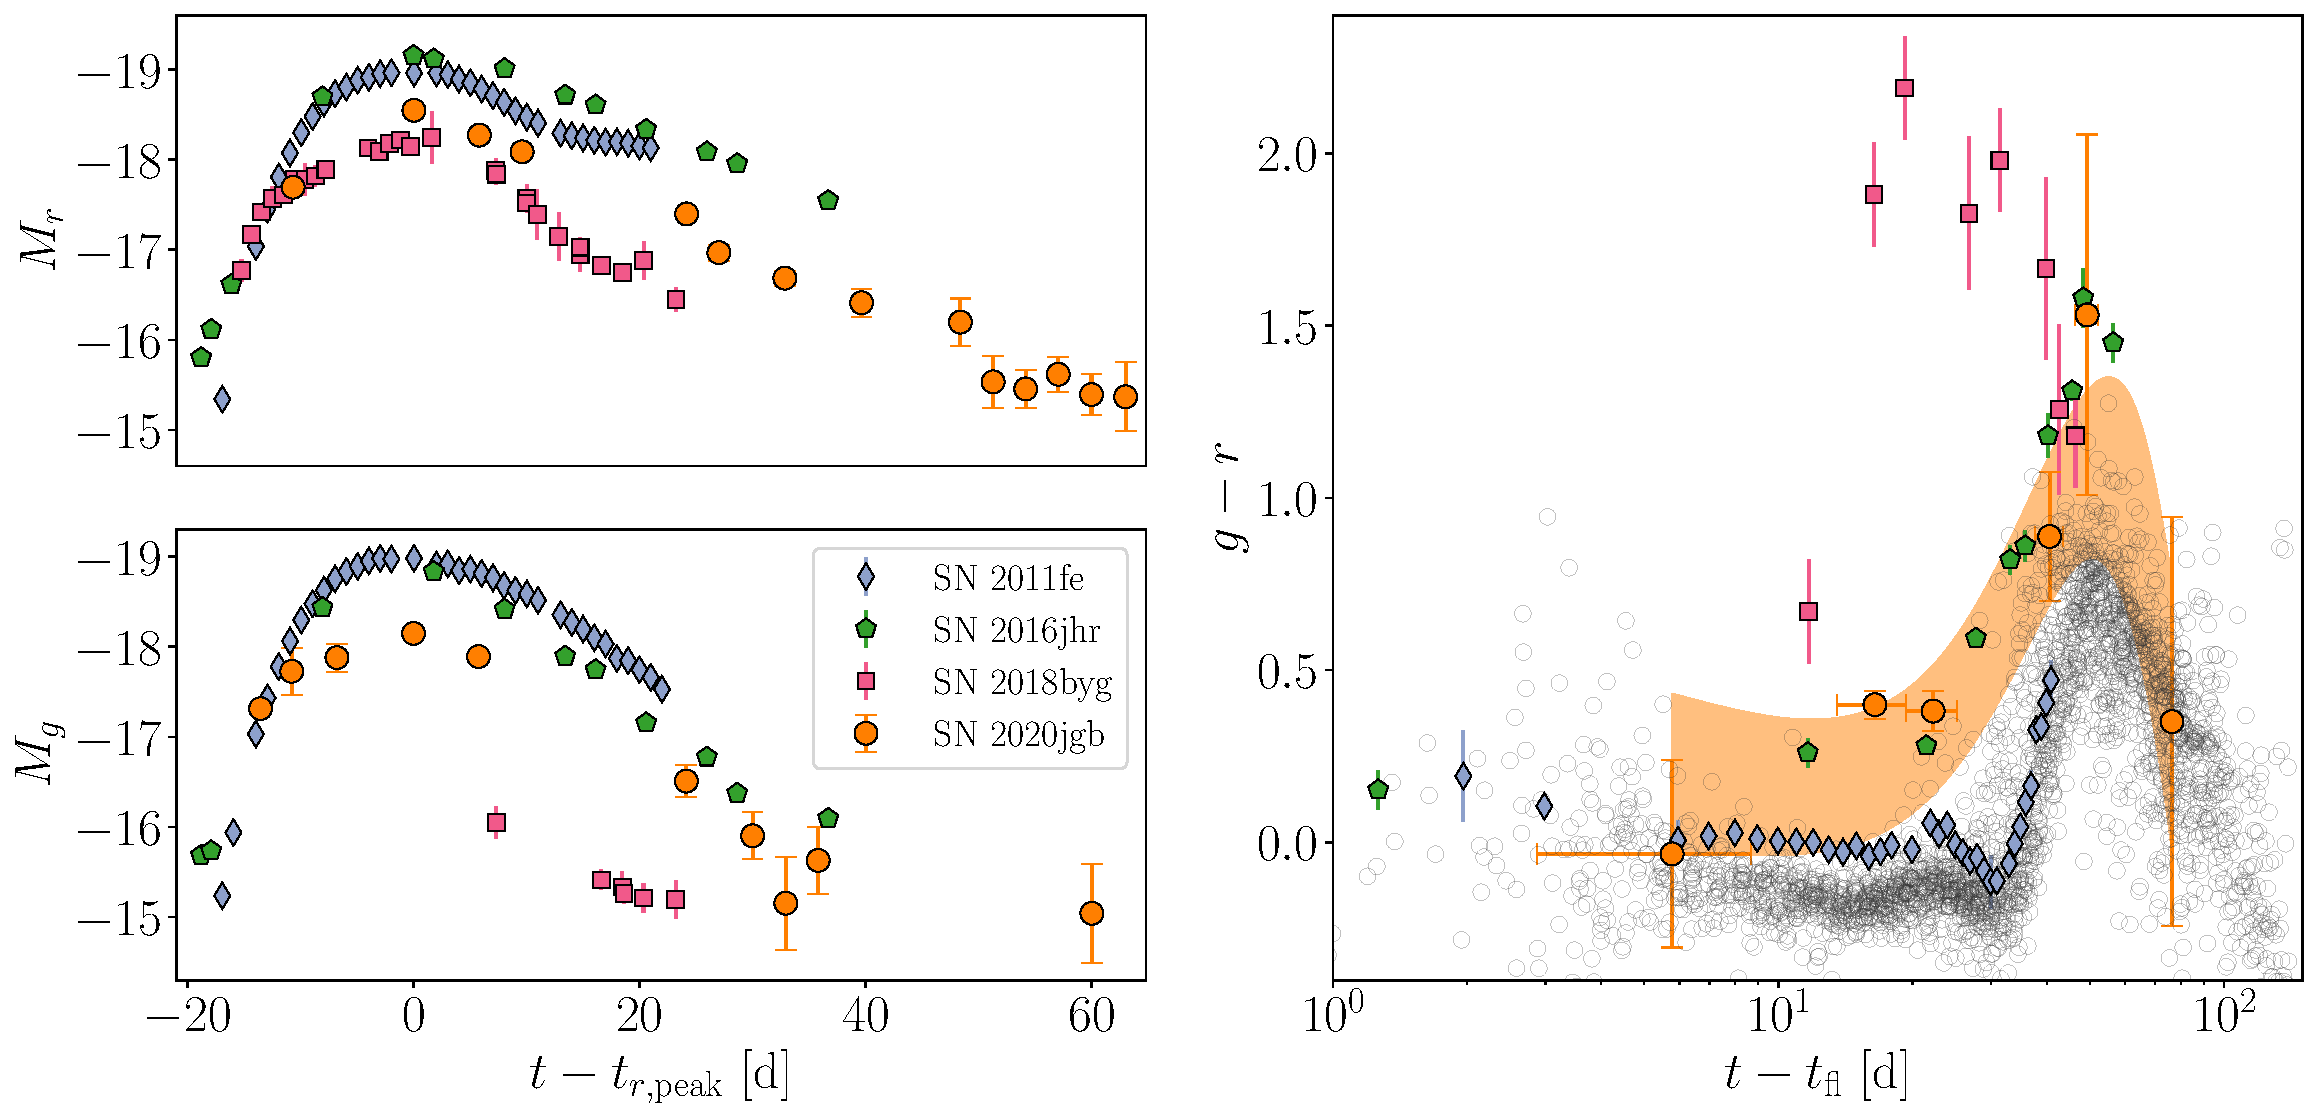
\includegraphics[width=\textwidth]{photometry.pdf}
    \caption{\textit{Left}: Comparison of the multi-color light curves  of \sn\ with the normal SN\,Ia SN\,2011fe, the thin shell DDet candidate SN\,2016jhr, and the thick shell DDet candidate SN\,2018byg. The upper (lower) panel shows the evolution in $g$-band ($r$-band) absolute magnitudes. \textit{Right}: comparison of $g-r$ color evolution to SN\,2011fe and SN\,2018byg, as well as 62 normal SNe Ia (open circles) with prompt observations within 5\,days of first light by ZTF \citep{Bulla2020}.}
    \label{fig:photometry}
\end{figure*}

\subsection{Optical Spectroscopy}\label{sec:optical_spec}
We obtained optical spectroscopic follow-up of the object from $\sim$$-10$\,days to $\sim$$+150$\,days relative to the $r_\mathrm{ZTF}$-band peak, using the Spectral Energy Distribution Machine \citep[SEDM;][]{SEDM_2018} on the automated 60\,inch telescope \citep[P60;][]{P60_2006} at Palomar Observatory, the Kast Double Spectrograph \citep{miller1994kast} at the Shane 3\,m Telescope, the Andalucia Faint Object Spectrograph and Camera (ALFOSC)\footnote{\url{https://www.not.iac.es/instruments/alfosc/}} installed at the Nordic Optical Telescope (NOT), the Double Beam Spectrograph (DBSP) on the 200\,inch Hale telescope \citep[P200;][]{P200_1982}, the Low Resolution Imaging Spectrograph (LRIS) on the Keck I telescope \citep{Keck_1995}. Spectra were reduced using standard procedures \citep[e.g.,][]{Matheson_2000}. Details of the spectroscopic observations are listed in Table~\ref{tab:spec}, and the spectral sequence is shown in Figure~\ref{fig:spec_evo}.

On 2022 March 31, two years after the transient faded, we also took a spectrum for its host galaxy using the DEep Imaging Multi-Object Spectrograph (DEIMOS) on the Keck II telescope \citep{DEIMOS_2003}, for a total integration time of 3200\,s. The spectra were reduced with the \texttt{PypeIt} Python package \citep{pypeit:joss_pub}.

\begin{deluxetable}{lrcccc}
\tabletypesize{\scriptsize}
\tablewidth{0pt}
\tablecaption{Spectroscopic Observations of \sn\label{tab:spectra}}
\tablehead{
\colhead{$t_\mathrm{obs}$} &
\colhead{Phase} &
\colhead{Telescope/} &
\colhead{$R$} &
\colhead{Range} &
\colhead{Air} \\
\colhead{(MJD)} &
\colhead{(d)} &
\colhead{Instrument} &
\colhead{$(\lambda/\Delta\lambda)$} &
\colhead{(\AA)} & 
\colhead{Mass}
}
\startdata
58,976.42 &  $-$9.7 & P60/SEDM & 100 & 3770--9220 & 1.23\\
58,982.12 & $-$4.2 & NOT/ALFOSC & 360 & 4000--9620 & 1.17\\
58,990.43 &  $+$3.9 & P60/SEDM & 100 & 3770--9220 &  1.23\\
58,997.44 & $+$10.7 & P60/SEDM & 100 & 3770--9220 &  1.29\\
58,998.41 & $+$11.6 & Shane/Kast & 1000? & 3620--10720 & 1.28\\
59,008.41 & $+$21.3 & P60/SEDM & 100 & 3770--9220 & 1.28\\
59,010.40 & $+$23.3 & P200/DBSP & 700 & 3200--9500 &  1.27\\
59,023.58 & $+$36.1 & Keck I/LRIS & 1100 & 3200--10250 & 2.04\\
59,107.29 & $+$117.3 & Keck I/LRIS & 1100 & 3200--10250 & 1.31\\
59,143.26 & $+$152.2 & Keck I/LRIS & 1100 & 3200--10250 & 2.16\\
\enddata
\tablecomments{Phase is measured relative to \trpeak\ in the host galaxy rest frame. The resolution $R$ is reported for the central region of the spectrum.}
\end{deluxetable}
\begin{figure*}
    \centering
    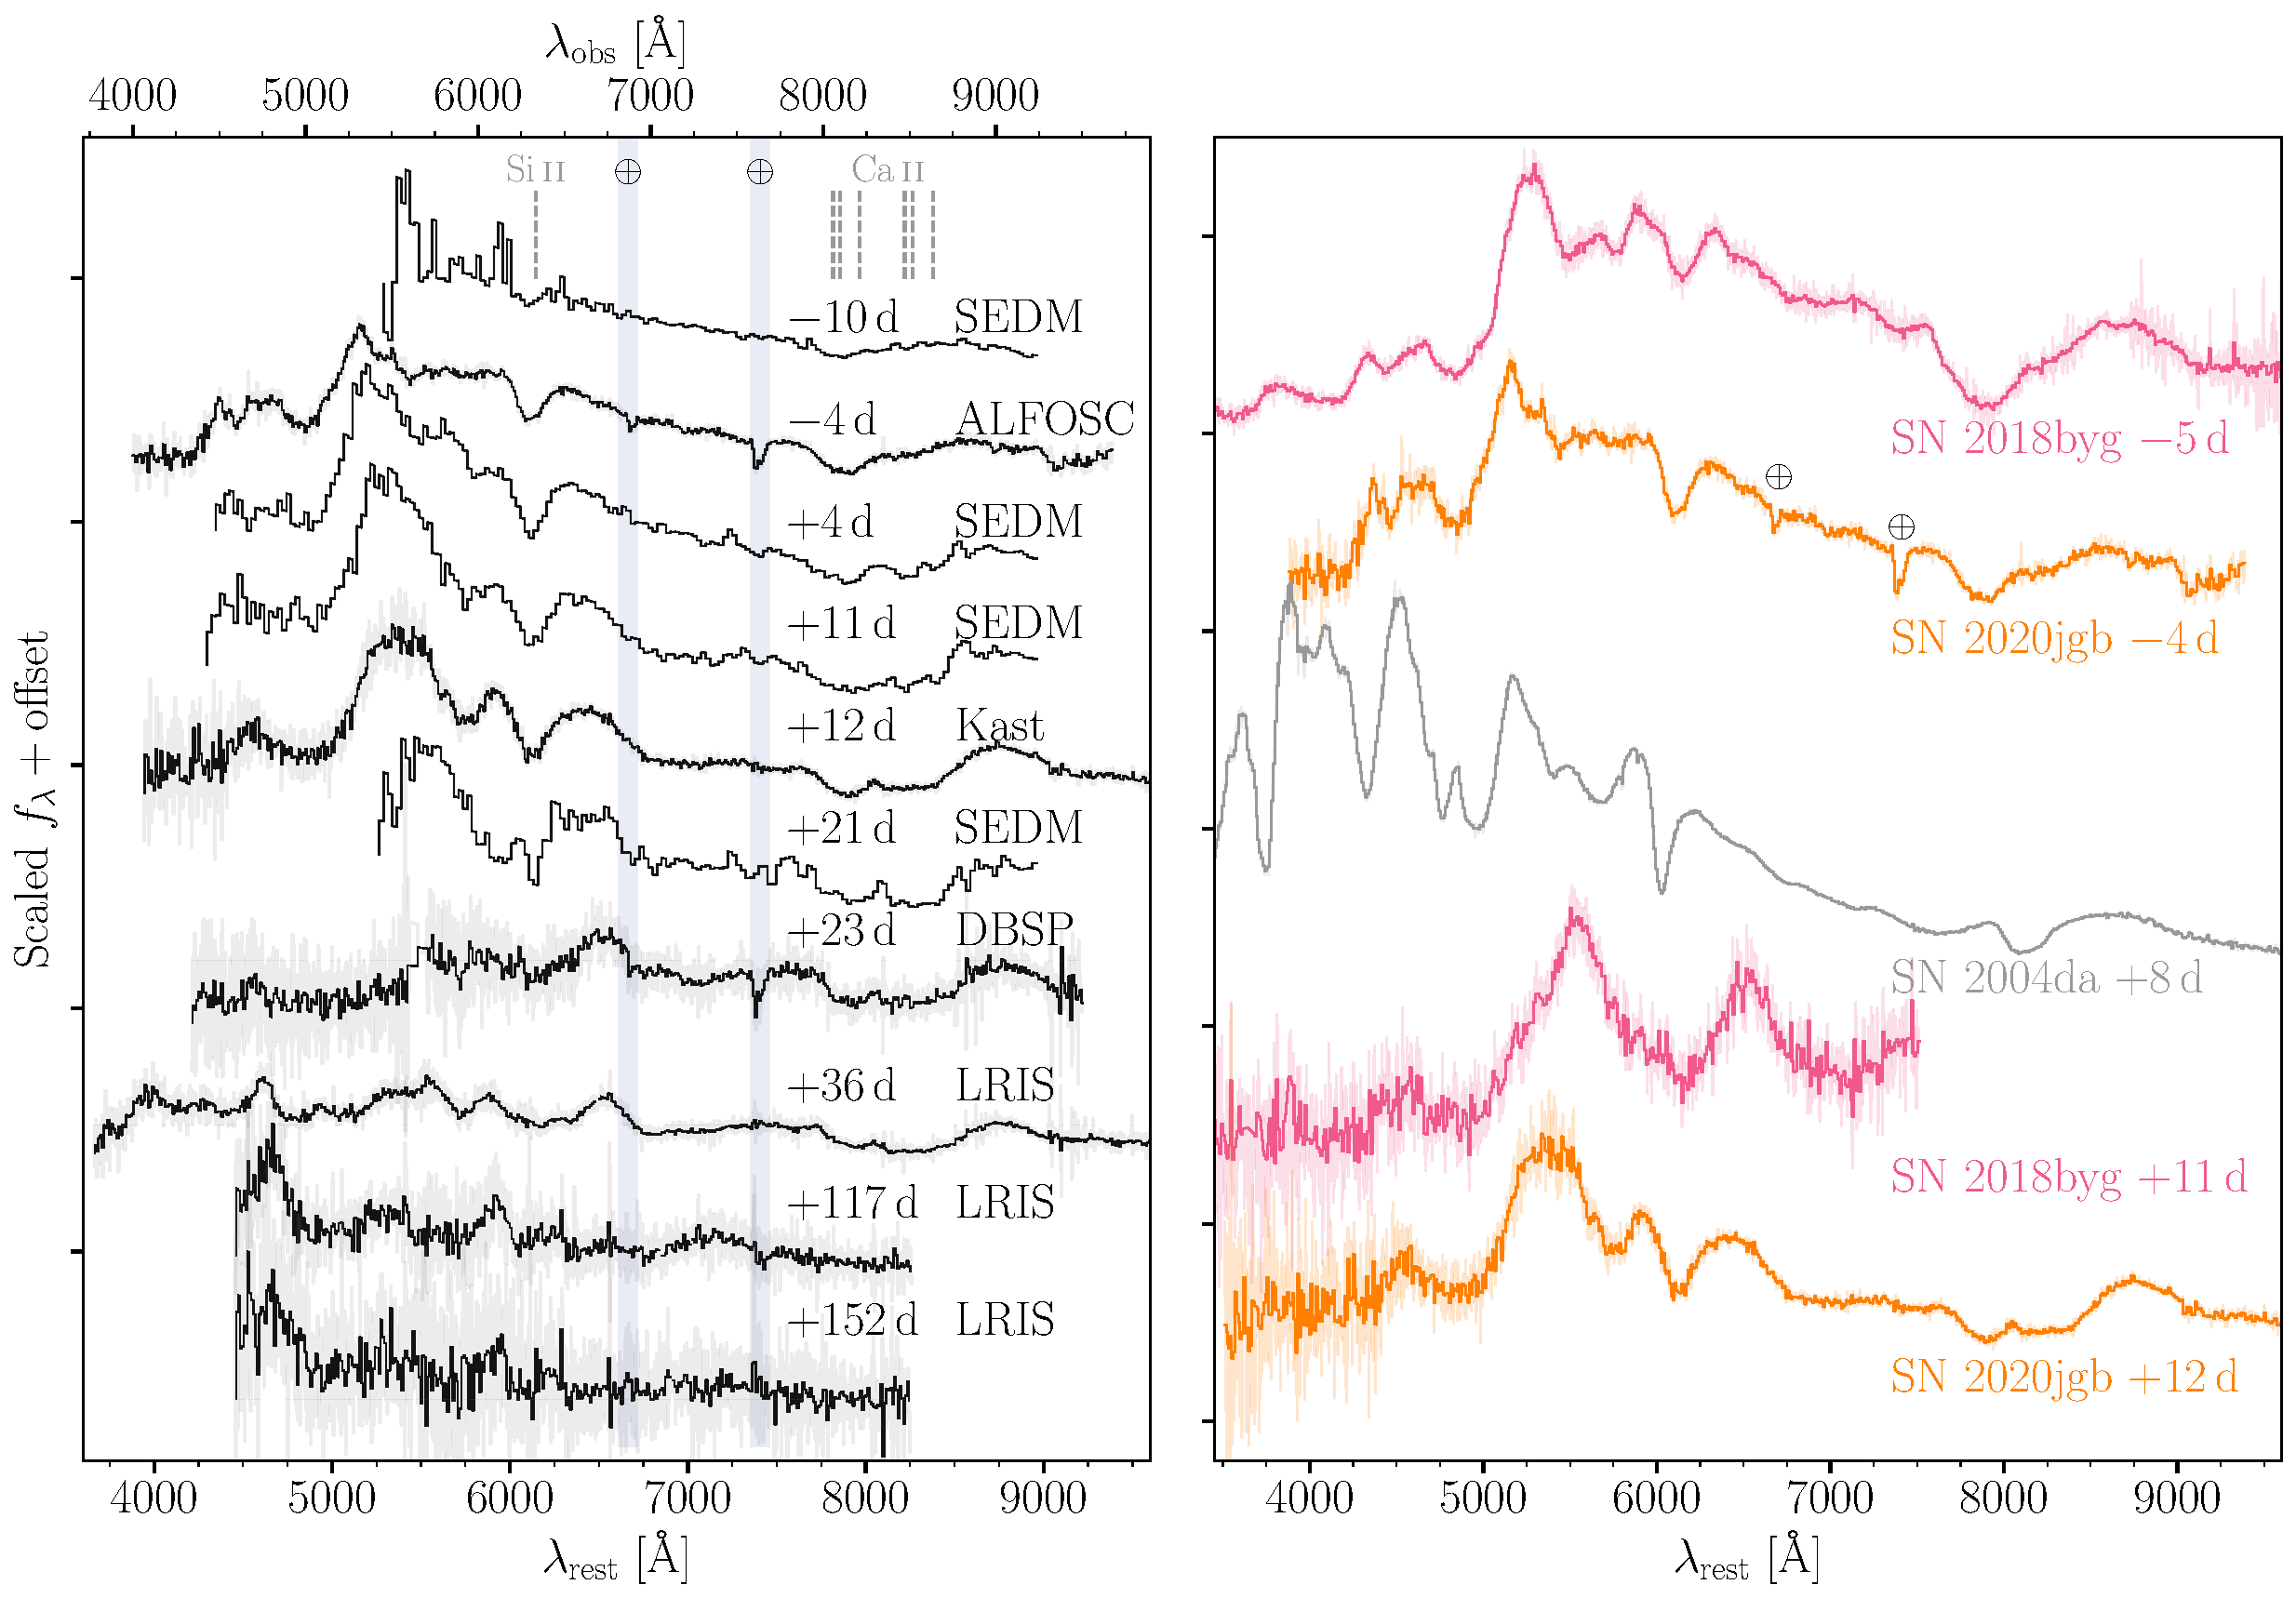
\includegraphics[width=\textwidth]{optical_spec_evolution.pdf}
    \caption{\textit{Left}: optical spectral sequence of \sn. Rest frame phases (days) relative to the $r_\mathrm{ZTF}$-band peak and instruments used are posted next to each spectrum. The spectra are after Galactic extinction correction are shown in grey. The black lines are binned spectra with a bin size of 10\,\r{A}, except for the SEDM spectra, whose resolution is lower than the bin size. In the last two spectra, we have subtracted the light from the host galaxy. Only regions with SNR $>2.5$ after binning are plotted. 
    \textit{Right}: spectral comparison with SN\,2018byg \citep[sub-luminous He-shell DDet;][]{de_18byg_2019} and SN\,2004da \citep[normal luminosity;][]{Silverman_2012}.}
    \label{fig:spec_evo}
\end{figure*}

\subsection{Near-infrared (NIR) Spectroscopy}
We obtained one NIR (0.8-2.5\,\micron) spectrum of \sn\ using the Gemini near-infrared spectrometer \citep[GNIRS;][]{GNIRS1998} on the Gemini North telescope on 2020 June 9 ($\sim$22\,days after $r_\mathrm{ZTF}$-band peak), for an integration time of 2400\,s. The GNIRS spectrum was reduced with \texttt{PypeIt}.

\begin{figure*}
    \centering
    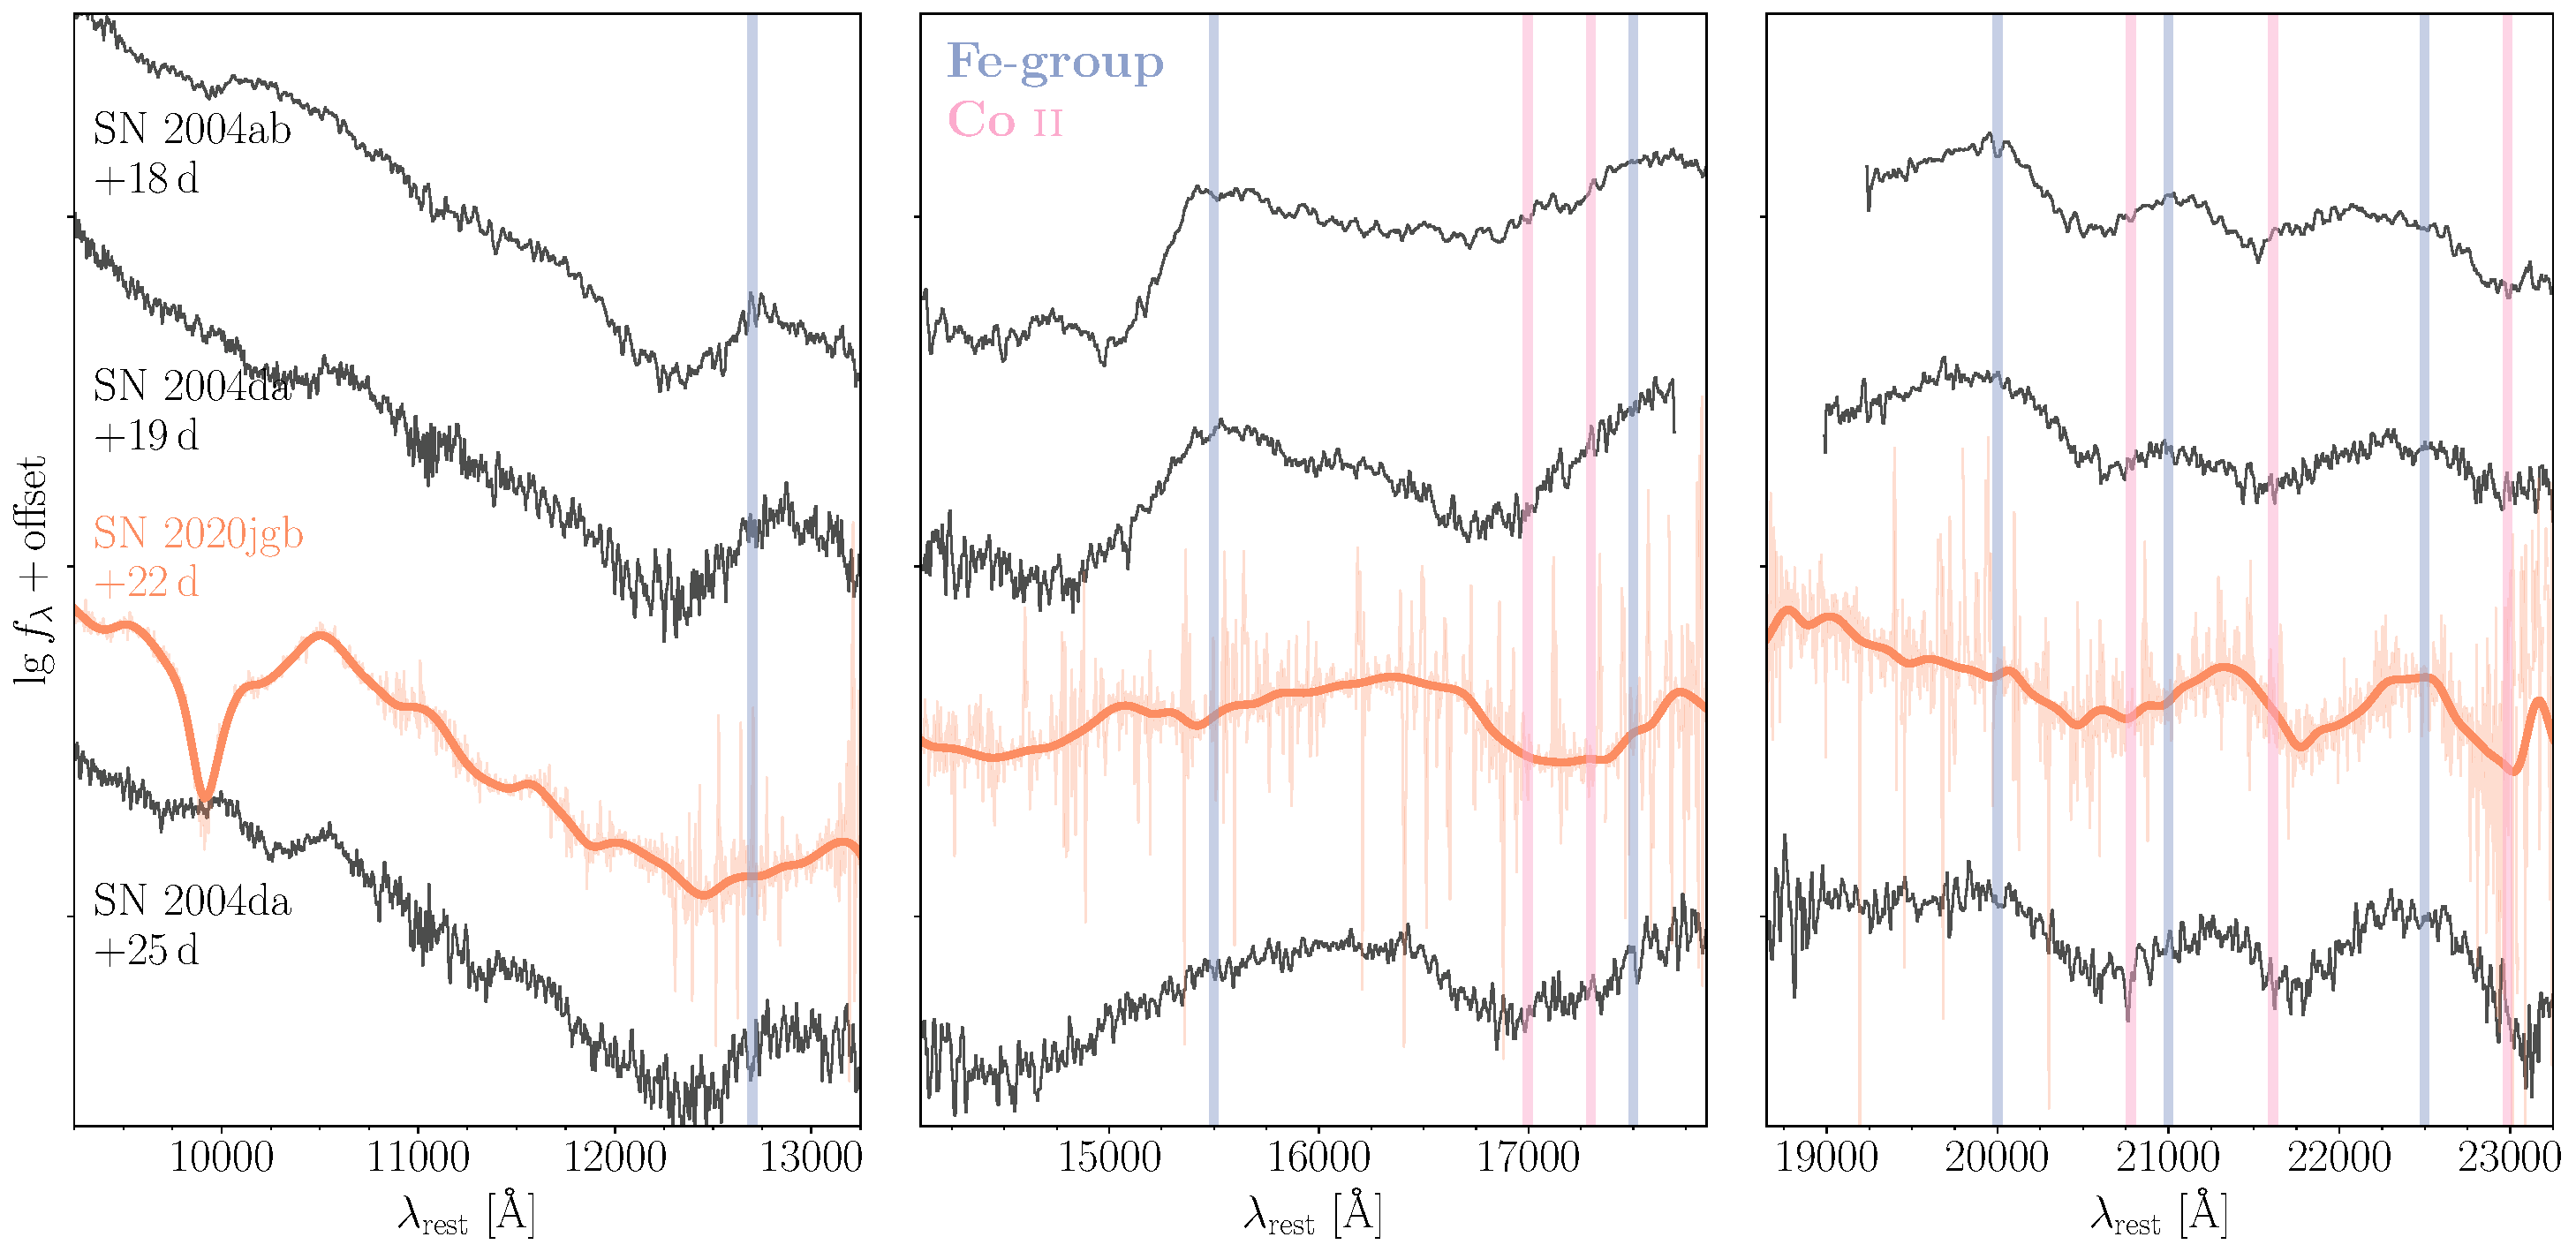
\includegraphics[width=\textwidth]{NIR_spec.pdf}
    \caption{The NIR spectra of \sn\ and two SNe Ia with normal maximum luminosity \citep[SN\,2004ab and SN\,2004da,][]{Marion2009_NIR}, taken about three weeks after the peak. For each spectrum, the continuum at $\gtrsim$1.2\,\micron\ is significantly reshaped by the Fe-group blanketing (emission features, blue vertical lines) and \ion{Co}{2} absorption (pink vertical lines). Spectra for SN\,2004ab and SN\,2004da are obtained from \citet{Marion2009_NIR}.}
    \label{fig:NIR_spec}
\end{figure*}

\section{Analysis} \label{sec:analysis}
\subsection{Photometric Properties}
\sn\ exhibited a fainter light curve than normal SNe Ia. In Figure~\ref{fig:photometry}, we compare the photometric properties of \sn\ with the nearby, well-observed SN\,2011fe \citep{Nugent_11fe_2011} and two He-shell DDet candidates, including the normal-luminosity thin shell candidate SN\,2016jhr \citep{jiang_16jhr_2017} and the sub-luminous thick shell candidate SN\,2018byg \citep{de_18byg_2019}, with available photometric data on the Open Supernova Catalog\footnote{See \url{https://github.com/astrocatalogs/supernovae}.} \citep{Guillochon_2017}. All these light curves have been corrected for Galactic reddening, while $K$-corrections have not been performed\footnote{These SNe were all observed in slightly different $g$- and $r$-bands.}. \chang{I thought 11fe peaked brighter than $-19$.} \adam{Double checked - essentially no Galactic extinction towards M101, so $M_g\approx18.98$\,mag. However, in the datafile from the open supernovae catalog, g-band light curves are referred to 2017MNRAS.472.3437G, where I couldn't find the data.}

While the observational coverage is sparse in the rise to maximum light, from Figure~\ref{fig:photometry} it is clear that \sn\ is less luminous than normal SNe\,Ia (e.g., SN\,2011fe). Furthermore, there is a flatter evolution in the $r_\mathrm{ZTF}$ evolution between $-14$\,d and maximum light for both \sn\ and SN\,2020jgb than there is for SN\,2011fe.  

In the right panel of Figure~\ref{fig:photometry}, we compare the color evolution ($g-r$) of these objects relative to the measured time of first light \tfl, accompanied by 62 normal SNe Ia (open circles) observed within 5 days of \tfl\ by ZTF \citep[from][]{Bulla2020}. For \sn\, the early rise of the light curve was not well sampled, so we estimate \tfl\ as the midpoint of the first detection and the last non-detection. We adopt an uncertainty on this estimate of 3\,days. 
All three DDet candidates are undoubtedly redder than normal SNe Ia. At peak light, \sn\ was not as red as the extreme case, SN\,2018byg ($g-r\approx2.2$\,mag), but exhibited a similar color as SN\,2016jhr ($g-r\approx0.5$\,mag).

\subsection{Optical Spectral properties}
In Figure~\ref{fig:spec_evo}, we show the optical spectral sequence of \sn, and compare its spectra with some other SNe Ia near peak luminosity. For the spectra obtained after +100\,d there is clear contamination from the host-galaxy, including the presence of narrow emission lines. For these spectra we subtract the galaxy light as measured in the DEIMOS spectrum from 2022 (see Section~\ref{sec:optical_spec}). The earliest spectrum was obtained by SEDM $\approx$10\,days before the $r_\mathrm{ZTF}$-band peak. We only show portions of the spectrum where the $\mathrm{SNR}>2.5$, where the continuum is almost featureless with some marginal detection of the \ion{Si}{2} $\lambda$6355 at $\approx$6100\,\r{A}, the trademark of SNe Ia. In subsequent spectra the \ion{Si}{2} features become more prominent and are clearly detected through +12\,d. We measure \ion{Si}{2} expansion velocities following a similar procedure as in \citet{Childress_2013,Childress_2014} and \citet{Maguire_2014}. The fitting region is selected by visual inspection. The continuum is assumed to be linear, and the absorption profile after the continuum normalization is assumed to be composed of double Gaussian profiles peaked at 6347\AA\ and 6371\AA. Within the model, the continuum flux density at the blue and red edges are free parameters for which we adopt a normal distribution as a prior. The mean and standard deviation for the normal are the observed flux density and its uncertainty, respectively, at each edge of the fitting region. Three more parameters (amplitude, mean velocity, logarithmic velocity dispersion) are used to characterize the double Gaussian profile, whose priors are set to be flat. This means the depths and widths of both peaks are forced to be the same, as \citet{Maguire_2014} has adopted in the optically thick regime. The priors of the three parameters are set to be flat. The Posteriors of the five parameters are sampled simultaneously with \texttt{emcee} \citep{emcee_2013} using the Markov chain Monte Carlo (MCMC) method. We find the mean expansion velocity is $\approx$11,500\,\kms near maximum light.

In many SNe Ia the \ion{Ca}{2} infrared triplet (IRT) absorption has two distinct components \citep{Mazzali_2005}, which are conventionally referred to as photospheric-velocity features (PVFs) and high-velocity features (HVFs). The PVFs originate from the main line-forming region with typical photospheric (i.e., bulk ejecta) velocities, while the HVFs are blueshifted to much shorter wavelengths, indicating significantly higher (by greater than $\sim$6000\,\kms) velocities than typical PVFs \citep{Silverman_HVF_2015}. Figure~\ref{fig:spec_evo} shows that \sn\ has prominent HVFs of \ion{Ca}{2} IRT. The HVFs are visible in our first spectrum of \sn, and remain prominent through $+36$\,days. Using a similar technique in modeling the \ion{Si}{2} features, we fit the HVFs and PVFs simultaneously. Both are fit by multiple Gaussian profiles assuming each line in the triplet can be approximated by the same profile (i.e., same amplitude and velocity dispersion). A best-fit expansion velocity of HVFs is $\gtrsim$26,000\,\kms. A clear delineation between the HVFs and PVFs is visible $\approx$4\,days before peak light. Since then we fit the broad absorption features with two different velocity components simultaneously. The velocity of HVFs slightly declines but stays above $\approx$24,000\,\kms, and the velocity of PVFs declines from $\approx$11,000\,\kms to $\approx$9,000\,\kms. As in normal SNe Ia, the relative strength between the HVFs and PVFs decreases with time. \chang{might be worth a figure - especially if we have this measured for several other DDet now}

The nebular phase spectra of \sn\ are dominated by the Fe-group elements, showing some enhancement in flux between $\approx$4500 and $\approx$6000\,\r{A}. We did not detect any emission feature related to [\ion{Ca}{2}] $\lambda\lambda$7291, 7324, which is a hallmark for Calcium-rich gap transients and is also prominent in a few DDet candidates \citep[e.g., SN\,2016hnk and SN\,2019ofm;][]{De_Ca-rich_2020}. 

The optical spectral evolution of \sn\ resembles that of SN\,2018byg, a sub-luminous DDet with a thick He-shell. At early times, both SNe were relatively blue and featureless with broad and shallow \ion{Ca}{2} IRT absorption. As they evolved closer to maximum light, they developed strong continuous absorption bluewards of $\approx$5000\,\r{A}, while the \ion{Si}{2} $\lambda$6355 and the \ion{Ca}{2} IRT became more prominent. \ion{S}{2} was not detected in either object. In the DDet scenario, a large amount of Fe-group elements will be synthesized in the outer regions of the ejecta, which will cause significant line-blanketing near maximum light \citep{Kromer_DD_2010, polin_observational_2019}, and also high velocity intermediate-mass elements like \ion{Ca}{2} \citep{Fink_DD_2010, Kromer_DD_2010}. The similarity between \sn\ and SN\,2018byg, makes \sn\ another promising DDet SN candidate. 

SN\,2004da is a normal SN\,Ia that shows similarities to \sn\ in the NIR (Section~\ref{sec:NIR_spec}), however, the two SNe are extremely different in the optical (Figure~\ref{fig:spec_evo}). From this comparison it is clear that \sn\ is not a normal SN\,Ia. 

\subsection{NIR Spectral properties}
\label{sec:NIR_spec}
The NIR spectrum of \sn\ is compared with two normal SNe Ia at a similar phase in Figure~\ref{fig:NIR_spec} \citep[data for SNe\,2004ab and 2004da from][]{Marion2009_NIR}. \sn\ shows a strong absorption feature at $\sim$0.99\,\micron, which is not seen in normal SNe Ia. This feature was still significant two weeks later, as detected by LRIS on Keck (see Figure~\ref{fig:hvf_comp}), though it was only partially covered. Aside from this prominent feature, \sn\ resembles normal SNe Ia in NIR band. The shape of the continuum redwards to $\approx$1.2\,\micron\ is significantly altered by line-blanketing from Fe-group elements. Just like normal SNe Ia, \sn\ shows an enhancement of flux at about 1.3, 1.55, 2.0, 2.1, and 2.25\,\micron, accompanied by several \ion{Co}{2} absorption lines. It is especially similar to SN\,2004da at +25\,days after maximum light as the steep increase in flux at $\approx$1.55\,\micron, known as the \textit{H}-band break \citep{Hsiao_CSP_2019}, has become less prominent.

In a sample of 15 spectra for normal SNe Ia between +14\,days and +75\,days after the peak light, not a single one shows such a prominent absorption features around 1\,\micron\ \citet{Marion2009_NIR}. We have investigated several potential identifications for this feature (see below), however, none of them provide a fully satisfying explanation.

The most tantalizing possibility is that the absorption is due to \ion{He}{1} $\lambda$10830. If \sn\ is a DDet SN, then unburned He could lead to observed absorption in the spectrum, as shown in the sub-Chandrasekhar-mass He-shell DDet models of \citet{Boyle2017_Helium}. Figure~\ref{fig:hvf_comp} shows that the 1\,\micron\ feature, if associated with \ion{He}{1} $\lambda$10830, has a high velocity ($\approx$26,000\,\kms), especially considering the phase of the SN. The \ion{Ca}{2} IRT also exhibits similarly high velocities at the same phase ($\approx$24,000\,\kms), suggesting it is not impossible to see very high absorption velocities at this phase. The expansion velocity in the ejecta is roughly linearly proportional to the radius, so such a high velocity indicates that both the \ion{Ca}{2} IRT and the tentative \ion{He}{1} absorption line form far outside the normal photosphere, which has a velocity of only $\approx$10,000\,\kms. In this sense, the He-shell DDet scenario, in which the unburnt helium is located in the outermost ejecta, is indeed supported.

We cannot claim an unambiguous detection of \ion{He}{1}, however, as our spectra lack definitive absorption from other \ion{He}{1} features that we would expect to be prominent, such as \ion{He}{1} $\lambda$20581. Considering a line velocity of $\approx$26,000\,\kms and a host galaxy redshift of 0.0309, this line will be blueshifted to $\approx$1.95\,\micron\ in the observer frame, so will be strongly blended by the strong telluric lines within 1.8-2.0\,\micron. After telluric correction, the signal to noise ratio reaches $\sim$5, with which we still cannot see any significant absorption feature. An upper limit of the equivalent width is determined to be $<$$2\%$ of the \ion{He}{1} $\lambda$10830 line, while theoretically, the 20581 line is supposed to be only a factor of 6-12 weaker, depending on temperature \citep{Marion2009_NIR}. Another fact is that the 1\,\micron\ feature is as strong as the \ion{He}{1} $\lambda$10830 in many helium-rich core-collapse supernovae, say, Type Ib supernovae, in which the \ion{He}{1} $\lambda$20581 line is weaker than the \ion{He}{1} $\lambda$10830 line yet still prominent \citep{CSP_Ibc_2022}. In one of the models in \citet{Boyle2017_Helium}, there is no obvious \ion{He}{1} $\lambda$20581 absorption in the synthetic spectra (see their Figure~7), but the model is intended to be representative for normal-luminosity SNe Ia. If the 1\,\micron\ feature is associated with \ion{He}{1}, it would be very unusual if the 2\,\micron\ feature is not seen at all, even if somehow blended by the telluric lines.

Other possible identifications include \ion{Mg}{2} $\lambda$10927, \ion{C}{1} $\lambda$10693, and \ion{Fe}{2} $\lambda$10500 \& $\lambda$10863. The \ion{Mg}{2} $\lambda$1.0927\,\micron\ line is prevalent in the NIR spectra of SNe Ia, but usually disappears within a week after peak \citep{Marion2009_NIR}, while the 1\,\micron\ feature was still visible over a month after the peak in the Keck LRIS spectrum. The required radial velocity is $\approx$30,000\,\kms, $\approx$20\% faster than the HVFs of \ion{Ca}{2} IRT at the same phase. While such a high velocity for \ion{Mg}{2} has never been seen in other SNe Ia, since high-velocity intermediate-mass elements like magnesium and calcium can be synthesized by the detonation of helium shell \citep{Shen_DD_2014}, the \ion{Mg}{2} origin of the 1\,\micron\ feature cannot be strictly ruled out. But if we attribute this 1\,\micron\ feature to high-velocity \ion{Mg}{2}, we would expect an even stronger \ion{Mg}{2} $\lambda$9227 line to be blueshifted to the red edge of the \ion{Ca}{2} IRT, which is not detected. Given the strength of the 1\,\micron\ feature, the \ion{Mg}{2} $\lambda$9227 line should not be completely obscured by the \ion{Ca}{2} IRT features. 

\ion{C}{1} $\lambda$10693 is not observed as frequently as \ion{Mg}{2} $\lambda$10927 in SNe\,Ia. \citet{Hsiao_CSP_2019} presented a sample of five SNe Ia with \ion{C}{1} detections, showing the \ion{C}{1} feature is strongest for fainter, fast-declining objects. However, in their sample, the \ion{C}{1} feature is a pre-maximum feature which fades away as the luminosity peaks, so the discrepancy in phase is large. The required expansion velocity $\approx$22,000\,\kms, which is overwhelmingly faster than the estimated carbon velocity for the sample in \citet{Hsiao_CSP_2019} ($\sim$10,000-12,000\,\kms), but still consistent with the HVFs of \ion{Ca}{2} IRT. Nonetheless, no significant carbon absorption is detected in the optical band.

The \ion{Fe}{2} features in SNe Ia usually start to develop roughly three weeks after the peak, which is about the same phase as we obtained our GNIRS spectrum. Two \ion{Fe}{2} lines, $\lambda$9998 and $\lambda$10500, are actually visible on the blue/red wings of the 1\,\micron\ feature. The \ion{Fe}{2} $\lambda$10863 line is not yet seen in the GNIRS spectrum. They correspond to an expansion velocity of $\approx$8,000\,\kms, which is consistent with the PVFs of the \ion{Ca}{2} IRT at the same epoch. They also match the same two lines for normal SNe Ia \citep{Marion2009_NIR}, making the identification more reliable. Obviously, these two \ion{Fe}{2} features are wider and shallower than the strong feature between them. We fit the 1\,\micron\ feature with three Gaussian profiles. Two of them are set to be the blueshifted \ion{Fe}{2} $\lambda$9998 and $\lambda$10500, and the other is an uncorrelated Gaussian profile which mainly describes the absorption in the center. We find that the shallower and wider \ion{Fe}{2} lines only make up $\sim$40\% of the total equivalent width, and the rest $\sim$60\% comes from the central feature, which cannot be accounted for by any \ion{Fe}{2} feature at the same velocity. Given the similarity of the Fe-group line-blanketing between the GNIRS spectrum with the spectrum of SN\,2004da at +25\,days, the distribution of Fe-group elements inside each supernova ejecta should be somehow similar as normal SNe Ia, so the central region of the 1\,\micron\ feature is not likely to be associated with \ion{Fe}{2} either.


\section{Discussion} \label{sec:discussion}
\subsection{Models} \label{sec:model}
{\it A few sentences from Abi describing the models.}

In Figure~\ref{fig:model}, we show the comparison of the photometric and spectroscopic features of \sn\ with DDet models from \citet{polin_observational_2019}. The peak luminosity reflects the total progenitor mass (C/O core $+$ He shell), and we find models with a total mass of $0.95\,\mathrm{M_\odot}$ generally reproduce the $r$-band peak brightness well. Thus in Figure~\ref{fig:model}, the total mass is fixed to be $0.95\,\mathrm{M_\odot}$ in all models. The overall $r$-band photometric evolution is best fit by the model with a $0.87\,\mathrm{M_\odot}$ C/O core and a $0.08\,\mathrm{M_\odot}$ He shell, while all three models underestimate the $g$-band brightness after the peak. This deviation may be attributed to a variety of factors on handling the explosion and radiative transfer. First, throughout the simulations we assume local thermodynamic equilibrium (LTE), which is not valid once the ejecta becomes optically thin. Typically the bulk ejecta of a sub-\Mch\ SNe Ia remains optically thick for $\sim$30\,days since the explosion. But in modeling the brightness in $g$-band, the LTE assumption is even more tricky, because the major opacity in $g$-band comes from the Fe-group line-blanketing in the outermost ejecta, where the optical depth may evolve differently from that at the photosphere. Hence the LTE condition may quickly become inapplicable. Furthermore, our 1-D He shell model is not capable to capture the multi-dimensional effects in the explosion such as asymmetries. The viewing angle is known to have a significant influence on the observed light curves \citep{Kromer_DD_2010, Sim_2012, Gronow_2020, Shen_2021}, especially in bluer bands where the line-blanketing depends sensitively on the distribution of He-shell ashes \citep{Shen_2021}. In previous studies on other DDet objects, the $g$-band brightness is systematically under-predicted shortly after the peak, despite the fact that redder bands can be fit decently \citep[e.g.][]{jiang_16jhr_2017,jacobson-galan_16hnk_2020}.

The model which best fits the photometry ($0.87\,\mathrm{M_\odot}+0.08\,\mathrm{M_\odot}$) also reproduces the major absorption features (e.g., Fe-group line-blanketing, \ion{Si}{2} $\lambda$6355, PVFs of \ion{Ca}{2} IRT) and the corresponding expansion velocities near the peak light. 
However, we are not able to fit the continua in $g$-, $r$-, and $z$-bands simultaneously, and the strong \ion{Ca}{2} HVFs are not seen in the synthetic spectrum. These discrepancies could also be due to the asymmetry in the DDet, that \sn\ was observed fairly close to the ignition point, where the abundances of Fe-group elements and high velocity calcium synthesized in the shell could be much higher than an angle-averaged 1-D model would predict.
In addition, the predicted \ion{Si}{2} $\lambda$5972 does not show up in the observed spectrum.

{\it Conclusions from the model comparison.}

\begin{figure*}
    \centering
    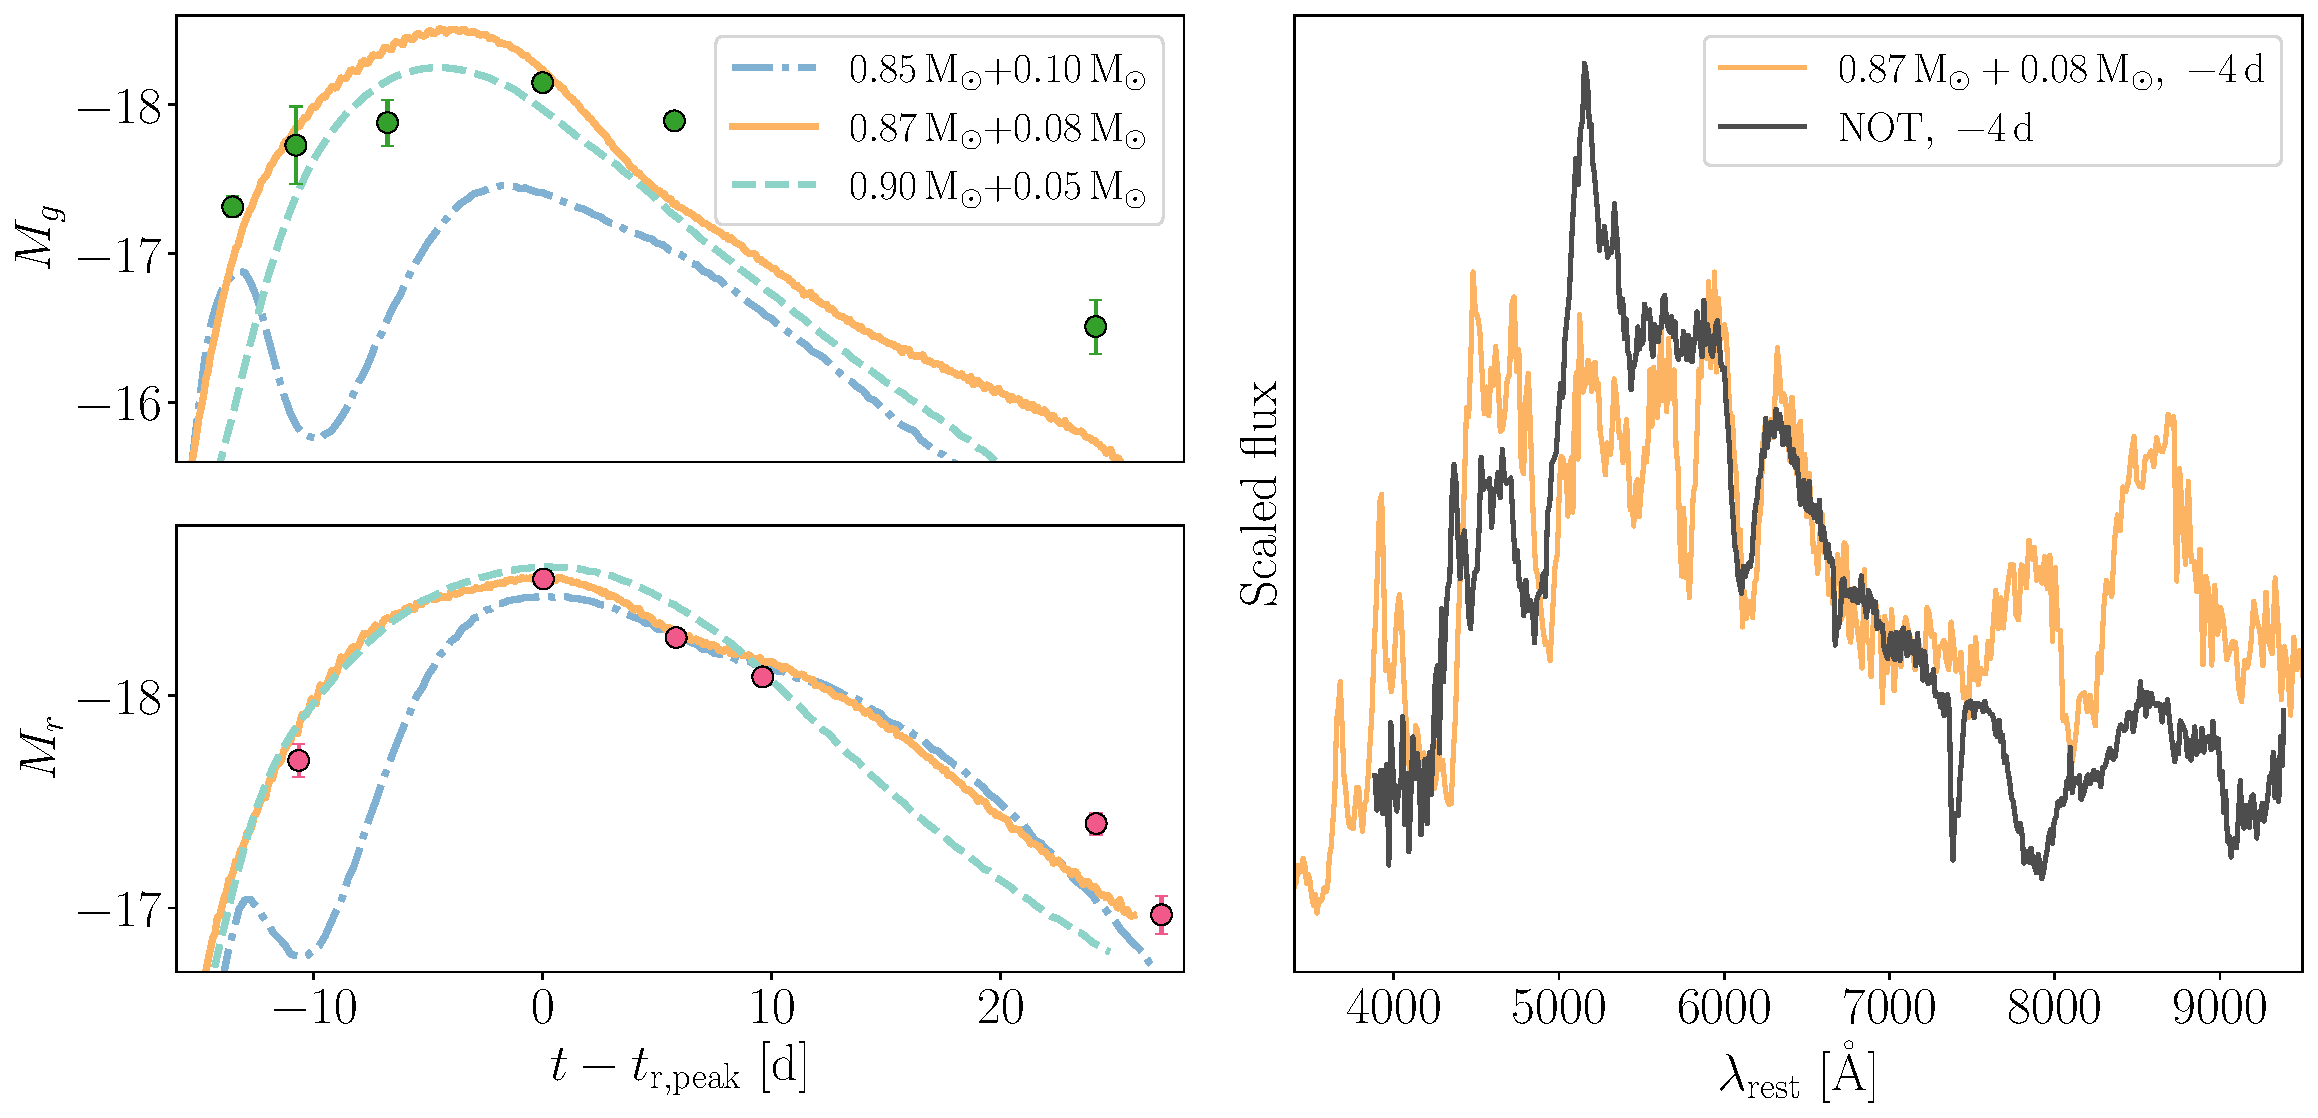
\includegraphics[width=\textwidth]{model.pdf}
    \caption{{\it Left:} Comparison of the photometric evolution of \sn\ with the He-shell DDet models from \citet{polin_observational_2019}. The model parameters are indicated in the legend as (C/O core mass $+$ He shell mass). The upper (lower) panel shows the evolution in $g$-band ($r$-band) absolute magnitudes. {\it Right:} Comparison of the spectrum of \sn\ with the $0.87\,\mathrm{M_\odot}$ C/O core $+$ $0.08\,\mathrm{M_\odot}$ He-shell DDet model before peak luminosity. Each spectrum is normalized by the median flux between 6500 and 7500\,\r{A}, and binned with a size of 10\,\r{A}. The synthetic spectrum 4\,days before the the $r$-band peak best matches the NOT spectrum (Galactic extinction corrected), which was obtained $\sim$4\,days before the $r_\mathrm{ZTF}$-band peak. All the phases have been rescaled to the host galaxy rest frame.}
    \label{fig:model}
\end{figure*}

\subsection{The 1\,\micron\ Feature} \label{sec:1um}
\begin{figure}
    \centering
    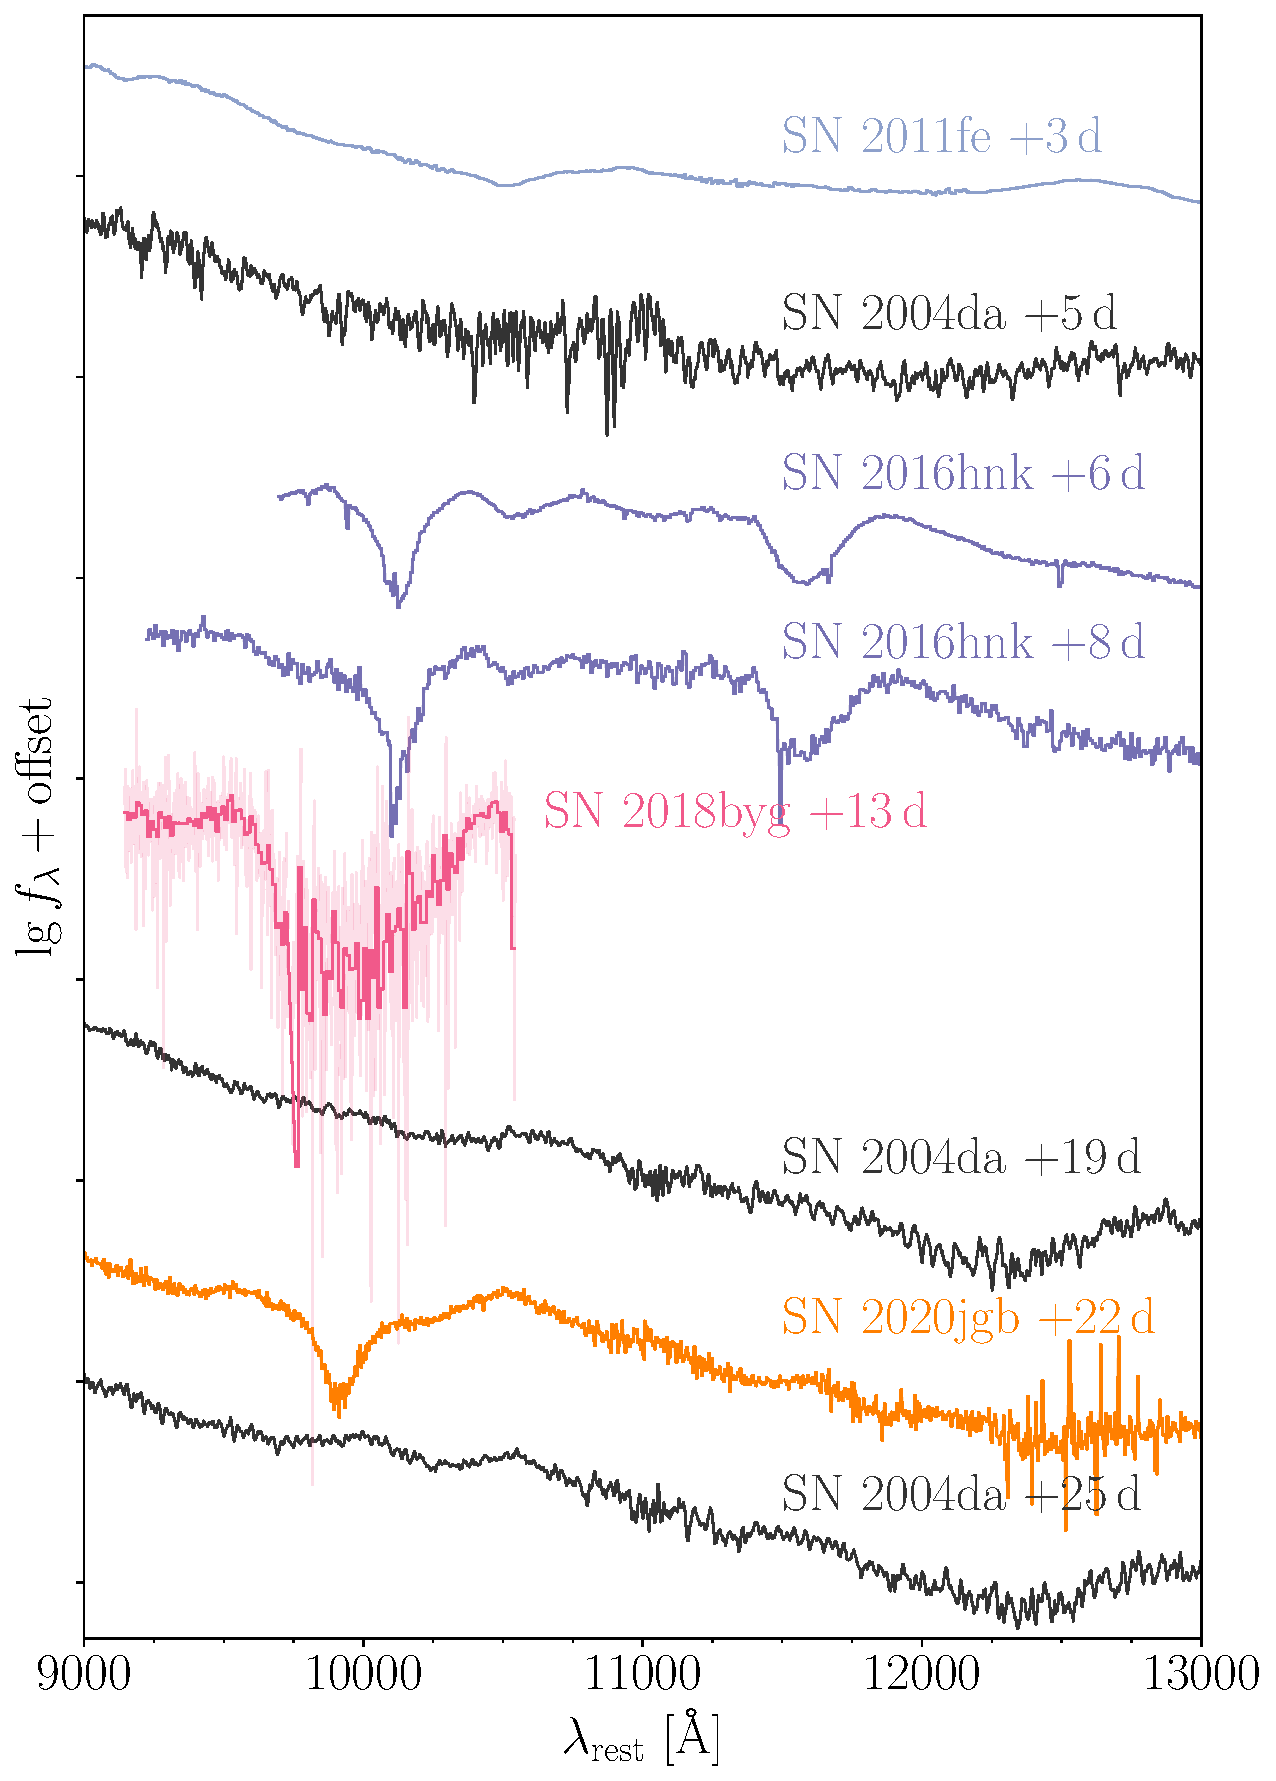
\includegraphics[width=\linewidth]{NIR_spec_comp.pdf}
    \caption{The NIR spectra (9000 to 13000\,\r{A}) of a few normal SNe Ia (SN\,2011fe and SN\,2004da) and three He-shell DDet candidates, which are all sub-luminous SNe Ia (SN\,2016hnk, SN\,2018byg, and this source, \sn). Other than the spectrum of SN\,2004da, all spectroscopic data are obtained from the WISEReP repository \citep{wiserep_2012}.}
    \label{fig:NIR_comp}
\end{figure}

While the nature of the 1\,\micron\ feature remains uncertain, other He-shell DDet candidates also seem to show similar complexity in this region. In the currently small sample of six candidates, three objects (SN\,2016jhr, SN\,2018aoz, and SN\,2019ofm) do not have any available NIR spectra, while the other three (at quite different phases though) all exhibit strong absorption features near 1\,\micron, as shown in Figure~\ref{fig:NIR_comp}. SN\,2016hnk has two deep absorption features around 1.02\,\micron\ and 1.17\,\micron, both are at a longer wavelength than the 1\micron\ feature in \sn. \citet{galbany_16hnk_2019} suggest both of them could be caused by \ion{Fe}{2}, though they are deeper than in other SNe Ia. The velocity of the 1.02\,\micron\ feature is $\approx$21,000\,\kms assuming a \ion{He}{1} $\lambda$10830 origin, which, just like \sn, is about the same as the HVFs of the \ion{Ca}{2} IRT in the optical spectra (see Figure~\ref{fig:hvf_comp}). The PVFs of the \ion{Ca}{2} IRT of both SNe have a similar expansion velocity of $\approx$10,000\,\kms. Such a consistency in velocities in also seen in SN\,2018byg (see Figure~\ref{fig:hvf_comp}). But given the exotic width and lower signal-to-noise ratio in the 1\,\micron\ feature, the exact line velocity is hard to determine. It is likely to be a mixture of several different lines. 

\citet{Dong_16dsg_2022} recently presented another thick He-shell DDet candidate, SN\,2016dsg, with an absorption line around $\sim$0.97-1.05\,\micron\ in a low-SNR NIR spectrum at $+16.6$\,days\footnote{SN\,2016dsg was discovered declining. The phase is relative to the discovery time.}. Assuming \ion{He}{1} $\lambda$10830 origin, the minimum of the absorption profile (at $\approx$1.03\,\micron, see Figure~4 in \citealp{Dong_16dsg_2022}) corresponds to an expansion velocity of $\approx$15,000\,\kms, lower than the 1\,\micron\ features in \sn, SN\,2016hnk, and SN\,2018byg assuming their \ion{He}{1} origin. Interestingly, SN\,2016dsg shows the least prominent HVFs of \ion{Ca}{2} IRT among the four, which also has a low velocity of $\approx$15,000\,\kms. Once again, the scenario where both the unburnt helium and the high velocity calcium are located at the outermost shell is favored.

Unfortunately, none of the spectra for SN\,2016dsg, SN\,2016hnk, or SN\,2018byg covers the 2\,\micron\ region, thus it is not possible to identify the presence of helium decisively. But if the 1\,\micron\ feature of the these objects are of the same origin, they are more likely to be correlated with the high velocity ejecta lying in the outmost region in the supernovae, because at least for \sn\ and SN\,2016hnk, the difference in their photospheric velocities cannot explain the discrepancy in their line velocities of the 1\,\micron\ feature. Then helium is still a promising candidate to cause strong absorption near 1\,\micron\ for these sub-luminous He-shell DDet SNe Ia. 

In conclusion, from all the He-shell DDet candidates with NIR spectra available, we have detected strong absorption features near 1\,\micron, which is not seen in normal SNe Ia. Indeed, these candidates have their NIR spectra taken at different epochs, hence each 1\,\micron\ feature can be of completely unrelated origin. Had they all originate from \ion{He}{1} $\lambda$10830, there would still be large diversity in the corresponding expansion velocities. This is to be confirmed in a more complete NIR spectral sequence in future He-shell DDet SNe Ia. Nonetheless, the apparently ubiquitous 1\,\micron\ features in various phases is possibly a distinctive attribute against normal SNe Ia.

\begin{figure*}
    \centering
    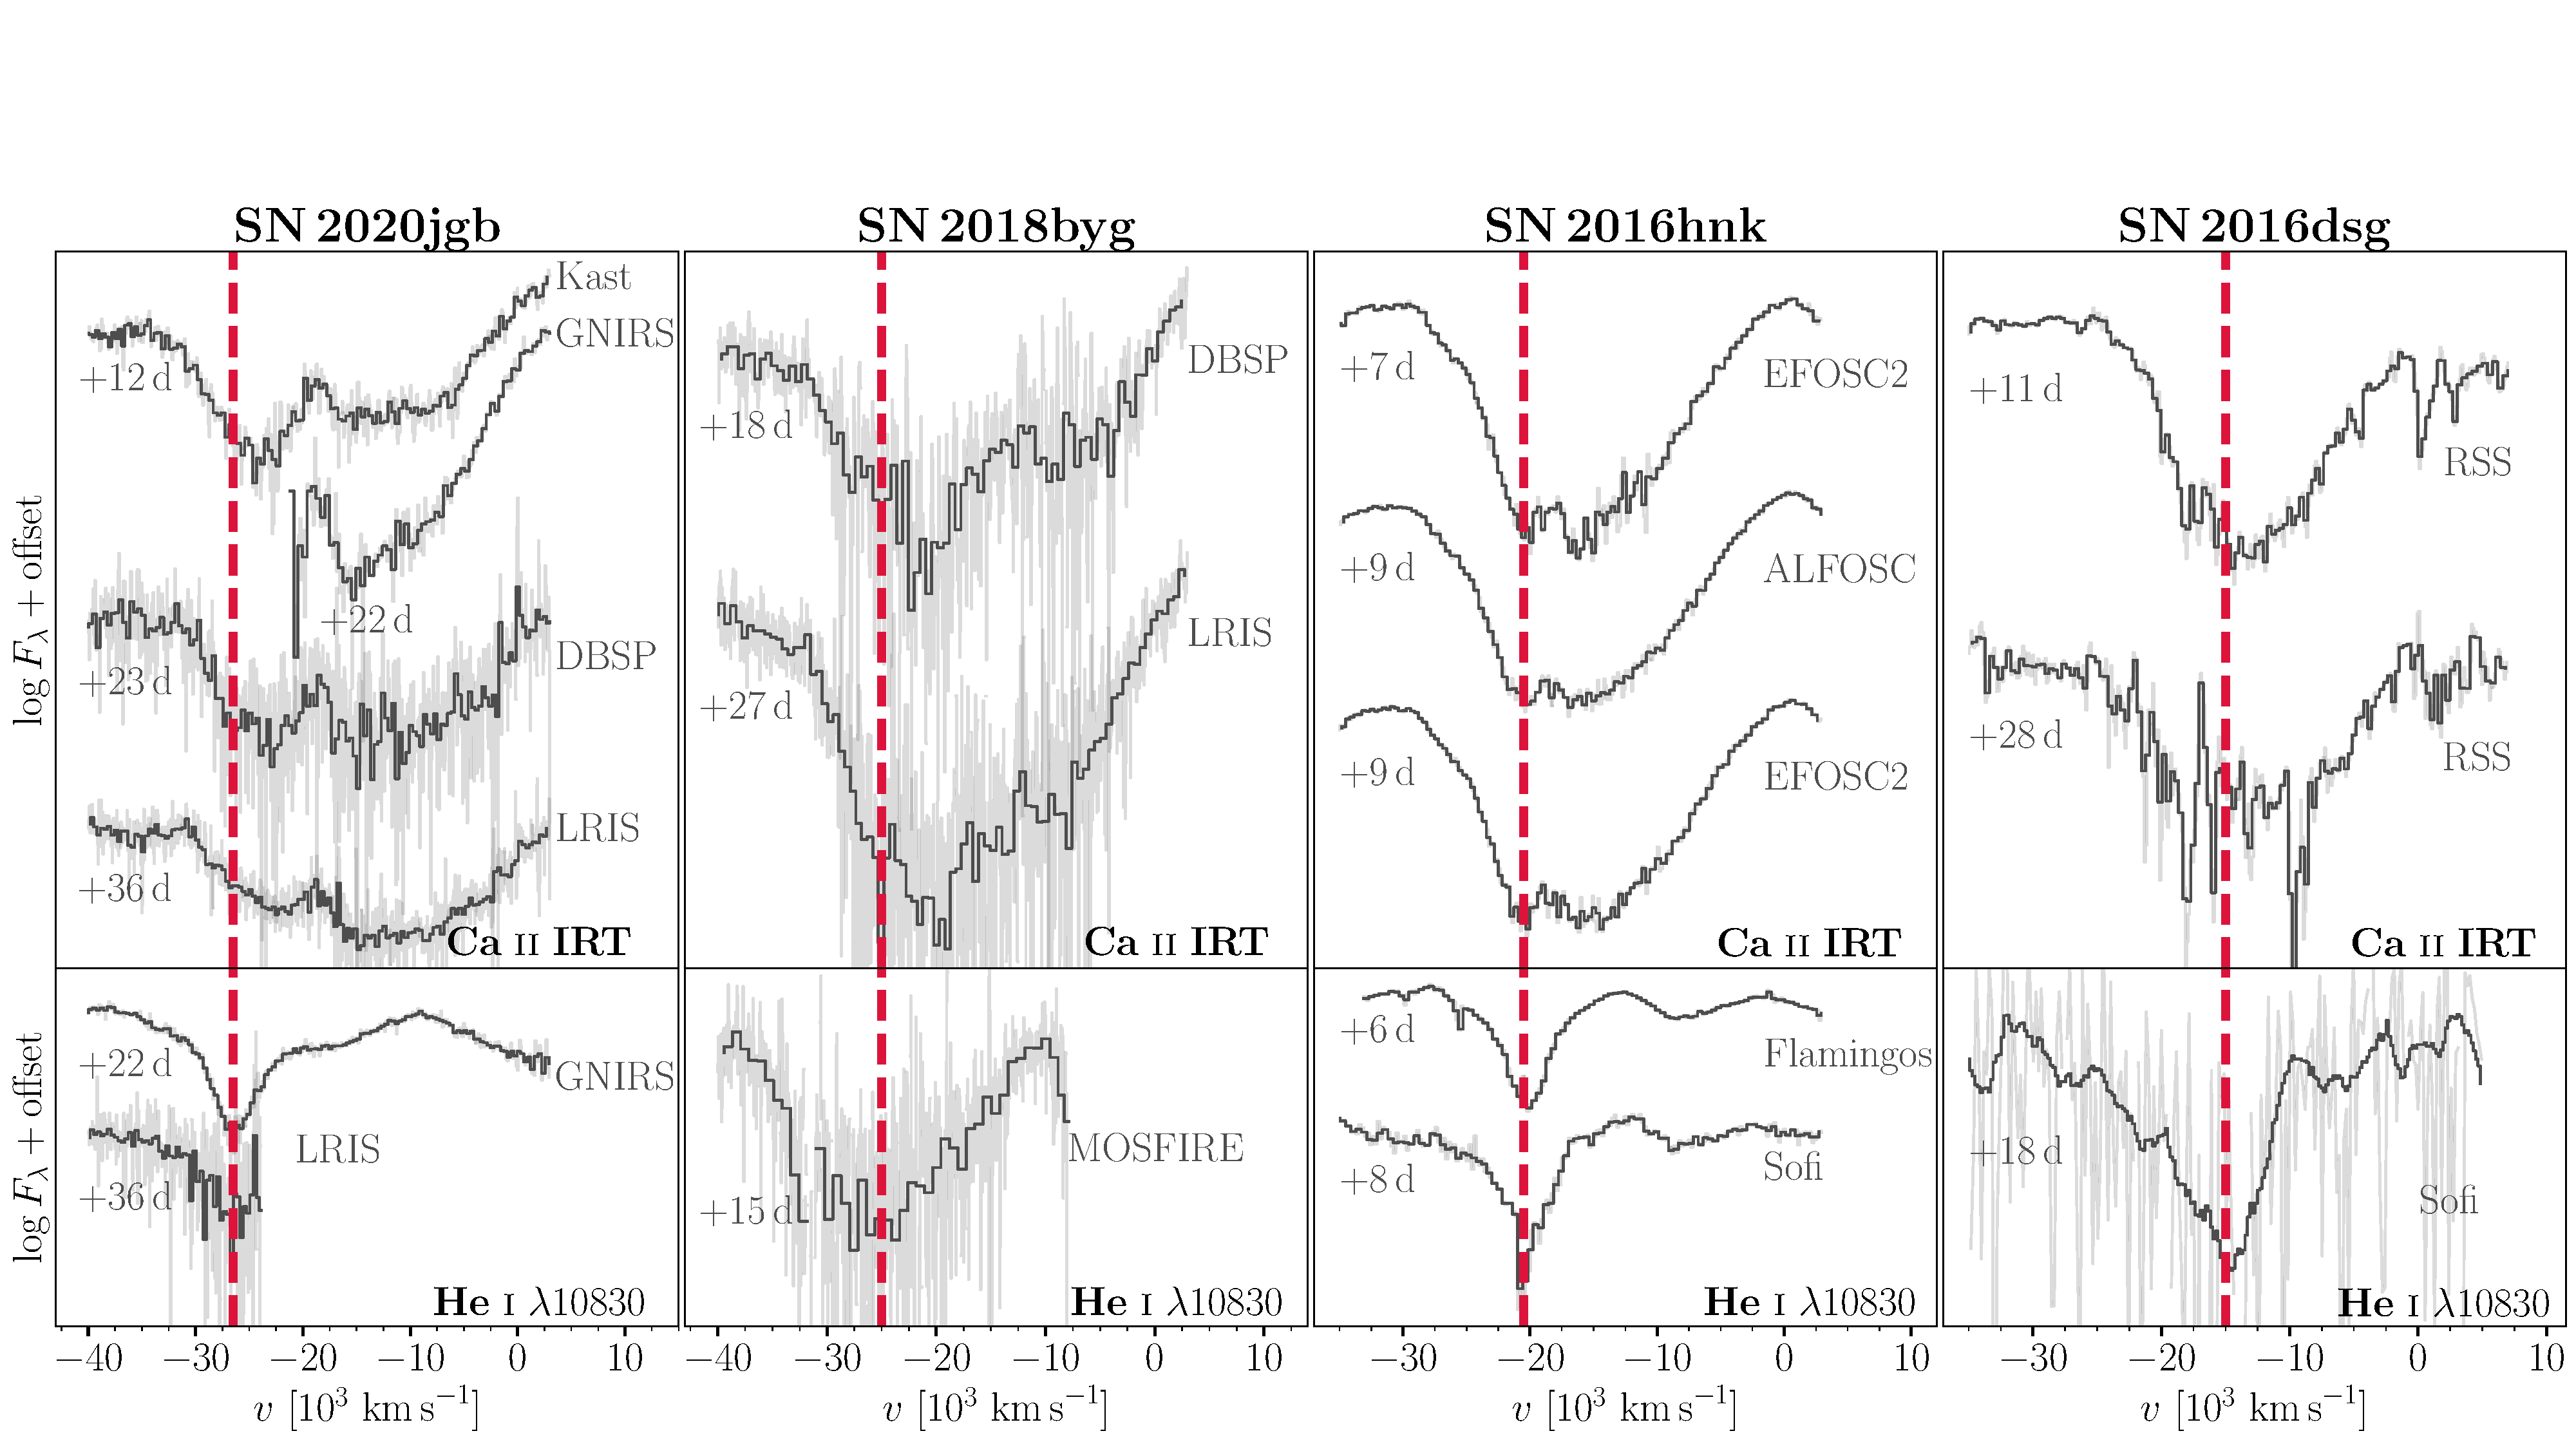
\includegraphics[width=\textwidth]{CaII_HeI_hvf.pdf}
    \caption{Spectra of \sn, SN\,2018byg, and SN\,2016hnk in the velocity space, comparing the \ion{Ca}{2} IRT absorption features (upper panels) and the 1\,\micron\ features assuming they are associated with \ion{He}{1} $\lambda$10830 (lower panels). The red dashed lines mark the minimum of each 1\,\micron\ feature. Data for SN\,2018byg and SN\,2016hnk are obtained from the WISEReP repository \citep{wiserep_2012}.}
    \label{fig:hvf_comp}
\end{figure*}

\subsection{Host Environments} \label{sec:host}
We model the stellar population of the host galaxy of \sn\ using \texttt{prospector} \citep{Johnson_prospector_2021}, a package for principled inference of stellar population properties using photometric and/or spectroscopic data. The input data included the Galactic extinction corrected DEIMOS spectrum, as well as the archival photometric data from the Panoramic Survey Telescope and Rapid Response System \citep[Pan-STARRS;][{\it r, i, z} Kron magnitudes]{PS1_2016}  and the VISTA Hemisphere Survey \citep[VHS;][J and $\mathrm{K}_\mathrm{s}$ Petrosian magnitudes]{VHS_2013} \chang{didn't we change to LS?} \adam{20jgb is outside the LS footprint}. In the best fit, the estimated stellar mass is $\log (M_*\,[\mathrm{M_\odot}])=7.79_{-0.06}^{+0.07}$, and the specific star-formation rate (sSFR) is $\log (\mathrm{sSFR}\,[\mathrm{yr}^{-1}])=-10.25_{-0.08}^{+0.09}$, with the uncertainties denoting the 68\% credible regions.

In Figure~\ref{fig:host}, we show the sSFR and the stellar mass for the host galaxies of six He-shell DDet candidates. Again using \texttt{prospector}, we fit the stellar properties for all the other candidates with optical spectra from the Sloan Digital Sky Survey \citep[SDSS;][]{York_2000} and photometry from the DESI Legacy Imaging Surveys \citep[][{\it g, r, z, $W_1$, $W_2$, $W_3$, $W_4$} magnitudes]{Dey_2019}. With mid-infrared photometry available, \texttt{prospector} can better estimate the overall dust extinction in the host galaxy and the contribution of an active galactic nucleus (AGN) to the spectral energy distribution (SED). Unfortunately, two (SN\,2016hnk and SN\,2019ofm) out of six hosts are close-by ($z\lesssim 0.03$) late-type galaxies with extended, spatially resolvable spiral structures. In both surveys, only photons from their red, concentrated bulges were fed to the detectors, while the lights from the blue, diffuse star-forming regions were completely missed. We would inevitably underestimate their SFR should we naively fit the SEDs from these surveys. Therefore, for the host of SN\,2016hnk, we adopt the results in \citet{galbany_16hnk_2019} as part of the PMAS/PPak Integral-field Supernova Hosts Compilation \citep[PISCO;][]{Galbany_PISCO_2018}, where the photons from the \ion{H}{2} regions in the spiral arms were also collected using integral field spectroscopy (IFS). For the host of SN\,2019ofm, there are no IFS data available, so we still show our best-fit stellar mass and sSFR in Figure~\ref{fig:host}, with the caveat that the sSFR should be regarded as a lower limit. The host of SN\,2018aoz (NGC\,3923) is a local ($z=0.00580$) early-type galaxy and is outside the SDSS footprint, so we adopt its stellar population properties from the Census of the Local Universe (CLU) catalog \adam{References?}.

With only a handful of He-shell DDet objects classified, they have been discovered in all kinds of host environments. Figure~\ref{fig:host} reveals that DDet SNe emerge in both star-forming and passive galaxies, which is true for both thin He-shell objects of normal luminosity (SN\,2016jhr in a star-forming host; SN\,2018aoz in a passive host) and thick He-shell, sub-luminous objects (SN\,2020jgb in a star-forming host; SN\,2018byg in a passive host), even when the natures of SN\,2016hnk and SN\,2019ofm remain ambiguous. There are also diversities in their locations in their hosts. SN\,2020jgb has a small projected physical offset ($\sim$0.2\,kpc) to the center of its host, a star-forming dwarf galaxy, so it is highly likely to originate from a young, star-forming environment. SN\,2016hnk has a moderate projected host offset ($\sim$4\,kpc) and a potential origin in an \ion{H}{2} region with ongoing star-formation \citep{galbany_16hnk_2019}. SN\,2019ofm has a large projected offset ($\sim$11\,kpc) but is still on the blue, diffuse spiral arm \adam{How can I refer to the DECaLS image?}. Other objects, including the recently discovered SN\,2016dsg and OGLE-2013-SN-079 \citep{Dong_16dsg_2022}, show large projected host offsets ($\gtrsim$10\,kpc) and lie in the galaxy outskirts, which usually indicates origin in old stellar population.

In this sense, the He-shell DDet sample resembles the normal SNe Ia population, which can occur in both star-forming and quenched galaxies \citep[e.g.,][]{Sullivan_2006, Smith_2012}, and is very different from some other types thermonuclear supernovae, such as Type-Iax supernovae (SNe Iax) which almost only appear in star-forming galaxies, or SN\,1991bg-like and SN\,2002es-like objects, which prefer old stellar environments \citep[see the review in][]{Jha_2019}. This favors the postulated sequence that He-shell DDet SNe may make up a substantial fraction of the normal SNe Ia, which is supported by studies on stellar metallicity observations \citep{Eitner_2022} or stellar population synthesis (\textbf{need references}).

The diversities in host environments indicate multiple formation channels in the He-shell DDet SNe population. Those in the star-forming environments, \sn\ being the most unambiguous example, could originate from some analogues of the two subdwarf B binaries with WD companions \citep{Geier_2013, Kupfer_2022} discovered in young stellar populations.
On the other hand, those with large host offsets could not be easily formed {\it in situ}. Similarly, many Ca-rich transients are also observed in remote locations \citep{Lunnan_2017}, for which some dynamical formation channels have been proposed. To reach the outskirts of galaxies, WD binaries would need to be hardened and ejected by globular clusters \citep{Shen_2019} or supermassive black holes \citep{Foley_2015} before explosions. Given that some Ca-rich transients show characteristic DDet properties \citep{de_Ca_rich_2020}, these channels may also be applicable to some of the He-shell DDet SNe. 

The robust detection of \sn\ in a star-forming region also agrees with independent studies on SNe Ia progenitors using stellar metallicity observations. \citet{de_los_reyes_manganese_2020}, by studying the manganese abundances in dwarf spheroidal satellites of the Milky Way, argue that sub-\Mch\ SNe Ia dominates the chemical evolution of a galaxy, while near-\Mch\ SNe tend to take over at later times. This indicates that observationally, sub-\Mch\ SNe Ia might have a stronger preference towards younger stellar populations than near-\Mch\ SNe Ia. Since He-shell DDet is one of the most favored channel to ignite a sub-\Mch\ WD, we would expect the majority of exploded SNe Ia in star-forming galaxies (at least the dwarfs) would undergo DDet. We note that while \sn\ is the first confirmed He-shell DDet SN in a star-forming dwarf, which indicates that thick shell DDet SNe might be intrinsically rare, the same may not be true for thin shell DDet SNe since they would look just as {\it normal} a few days after explosions \citep{Ni_2022}. Unfortunately, few of them are observed in such an early phase to date (SN\,2016jhr and SN\,2018aoz being two of them), thus we might have missed a great number of He-shell DDet SNe. With more efficient time domain surveys kicking in in the near future and prompt follow-up observations being increasingly available, a systematic studies on the infant SNe Ia will help confirm this implication.
\begin{figure}
    \centering
    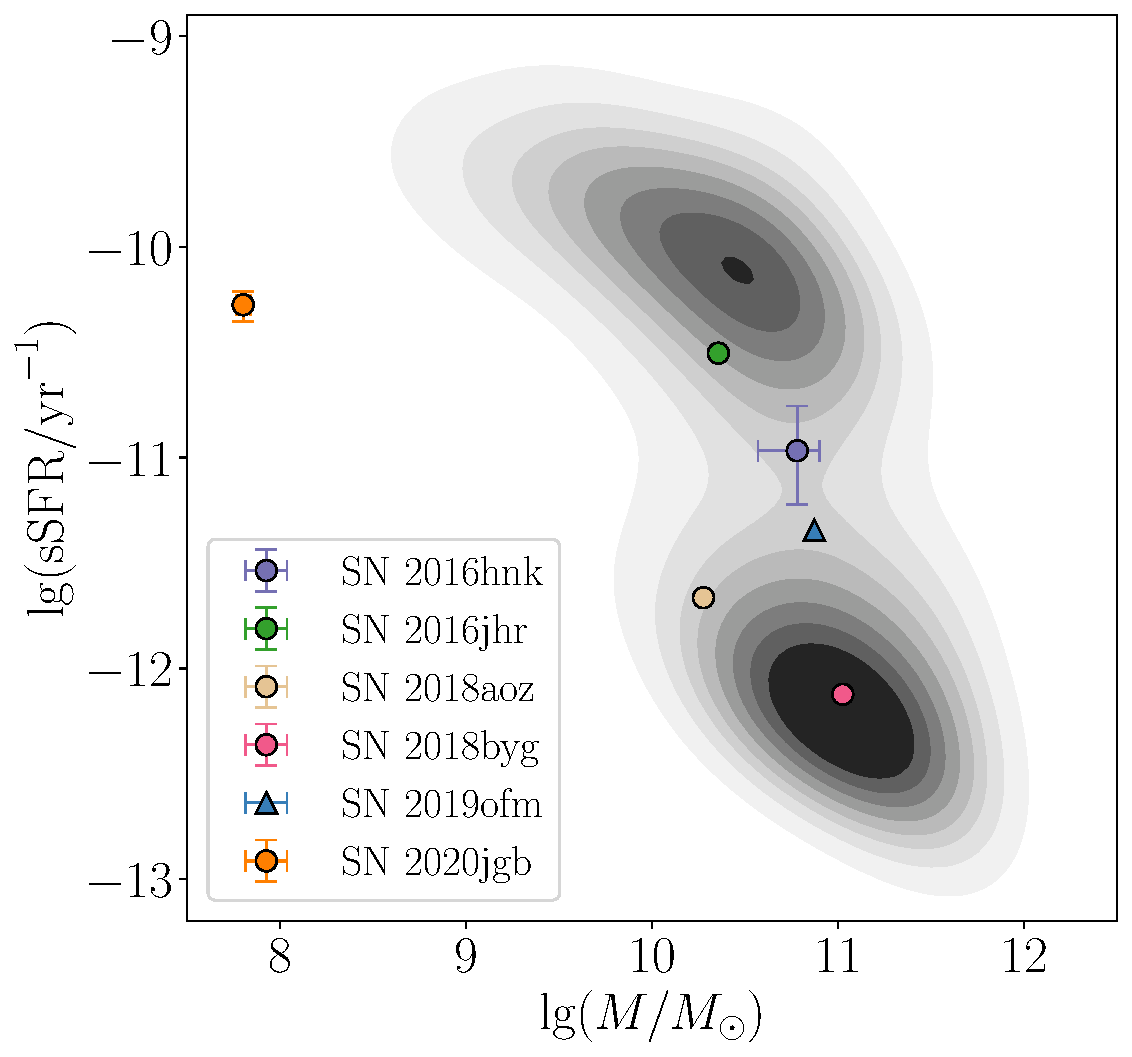
\includegraphics[width=\linewidth]{host.pdf}
    \caption{The specific star-formation rate (sSFR) and the stellar mass for the host galaxies of He-shell DDet candidates. The properties for the hosts of SN\,2016hnk and SN\,2018aoz are taken from \citet{galbany_16hnk_2019} and the CLU catalog \adam{References?}, respectively. For the sSFR in the host of SN\,2019ofm, only a lower limit is shown (the triangle). The background is a sample of galaxies from the SDSS MPA-JHU DR8 catalog \citep{Kauffmann_SDSS_2003,Brinchmann_SDSS_2004}. Galaxies with BPT classification as AGNs or LINERs are excluded, since certain spectral features (e.g., H$\alpha$ emission) due to nuclear activities might be misinterpreted as star formation.}
    \label{fig:host}
\end{figure}

\section{Conclusions} \label{sec:conclusion}
In the paper, we have presented the observations of \sn, a peculiar SN Ia. Putting together its low luminosity, red $g-r$ color, and strong line-blanketing in the spectra near peak light, we show it bears a high degree of resemblance to SN\,2018byg \citep{de_18byg_2019}, whose observational properties could be explained by the detonation of a shell of helium on a sub-\Mch WD. Fitting the light curves of \sn\ to a grid of models in \citet{polin_observational_2019}, we show a $\approx$0.87\,$\mathrm{M_\odot}$ WD beneath a $\approx$0.08\,$\mathrm{M_\odot}$ He-shell would be a reasonable estimate on its progenitor properties.

A high-SNR NIR spectrum obtained three weeks after the peak light shows a prominent absorption feature near 1\,\micron, which could be produced by the unburnt helium (\ion{He}{1} $\lambda$10830) in the outermost ejecta expanding at a high velocity ($\approx$26,000\,\kms). At the same epoch, the \ion{Ca}{2} IRT also exhibits similarly high velocities ($\approx$24,000\,\kms). By now, we have a very small sample of four candidate He-shell DDet SNe which have NIR spectra observed. Interestingly, all of them show deep absorption features near 1\,\micron, which, if assumed to have a helium origin, would be expanding very a similar HVFs velocity of \ion{Ca}{2} IRT, despite the huge diversity in velocities (from $\approx$15,000\,\kms in SN\,2016dsg to $\approx$24,000\,\kms in \sn). If it is the unburnt helium and the newly synthesized calcium from the He-shell that produce these line features, such a consistency in the expansion rates of different absorption lines would be naturally explained. However, we could not find unambiguous evidence for other \ion{He}{1} absorption, such as \ion{He}{1} $\lambda$20581, so we are not drawing a definitive conclusion on helium detection in \sn. Nonetheless, we discuss other potential strong lines (\ion{Mg}{2}, \ion{C}{1}, \ion{Fe}{2}) that may cause the 1\,\micron\ feature, but have found them also not that likely. Helium is still the most promising candidate for the apparently ubiquitous 1\,\micron\ features.

This paper provides a framework for robust \ion{He}{1} detection in He-shell DDet SNe. 
Ideally, one will need a NIR spectrum covering both the 1\,\micron\ and 2\,\micron\ regions in search of the \ion{He}{1} $\lambda$10830 and $\lambda$20581 features. Since the \ion{He}{1} $\lambda$20581 is weaker or even invisible when the He-shell is thin \citep{Boyle2017_Helium}, and could be blended with strong telluric lines, one should not always expect to see significant absorption features near 2\,\micron. For transients showing a clear 1\,\micron\ feature, one can calculate the required velocity assuming an origin in \ion{He}{1} $\lambda$10830 and check if it is comparable with the HVFs velocity in the \ion{Ca}{2} IRT absorption at a similar phase. While the detonation recipe in a DDet model and the viewing angles would all affect the observed \ion{He}{1}/\ion{Ca}{2} velocity, we still expect the elements along the line-of-sight to expand at a similar pace, if they all have a He-shell origin. Excluding the possibility of other strong lines is also necessary. If the NIR spectrum is obtained before the peak of the SN, strong \ion{Mg}{2} and \ion{C}{1} absorption \citep{Hsiao_CSP_2019} would be possible contaminants. Otherwise if the 1\micron\ feature is seen in the transitional-phase spectrum when the inner region of the SNe become visible, we need to carefully rule out the possibility of \ion{Fe}{2} origin \citep{Marion2009_NIR}.

The He-shell DDet SNe in the tiny sample show diversities in various observational properties, including the peak luminosity, color evolution, chemical abundances and line velocities, which could be explained by a large variety of He-shell masses, WD masses, viewing angles, and the initial chemical compositions in the shell. In addition, they are discovered in both old and young stellar populations, \sn\ being the first unambiguous thick He-shell DDet candidate detected in a star-forming galaxy, similar to the normal SNe Ia population. This is in favor of the scenario that a significant fraction of normal SNe Ia are triggered by He-shell DDet. Multiple formation channels and progenitor systems may be required to explain the He-shell DDet population.

\begin{acknowledgements}
\end{acknowledgements}

\facility{PO:1.2m (ZTF), PO:1.5m (SEDM), Hale (DBSP), NOT (ALFOSC), Shane (Kast Double spectrograph), Keck:I (LRIS), Keck:II (DEIMOS), Gemini:Gillett (GNIRS)}

\software{\texttt{astropy} \citep{Astropy_2013, Astropy_2018}, \texttt{emcee} \citep{emcee_2013}, \texttt{matplotlib} \citep{Matplotlib_2007}, \texttt{prospector} \citep{Johnson_prospector_2021}, \texttt{PypeIt} \citep{pypeit:zenodo}, \texttt{scikit-learn} \citep{scikit-learn}, \texttt{scipy} \citep{Scipy_2020}, \texttt{seaborn} \citep{Waskom_seaborn_2021}.}

\bibliography{SN2020jgb, software}
\bibliographystyle{aasjournal}

%% This command is needed to show the entire author+affiliation list when
%% the collaboration and author truncation commands are used.  It has to
%% go at the end of the manuscript.
%\allauthors

%% Include this line if you are using the \added, \replaced, \deleted
%% commands to see a summary list of all changes at the end of the article.
%\listofchanges

\end{document}

% End of file `sample631.tex'.
